% You can switch between one-sided printing (option 'oneside') and two-sided printing with different margines (option 'twoside') here.
\documentclass[a4paper,oneside]{csthesis}

% package to be able to use special characters
\usepackage[utf8]{inputenc}

% Sophisticated math package
\usepackage{amsmath}

% Special symbols
\usepackage{amssymb}

% nicely render theorems and proofs
\usepackage[standard,thmmarks,amsmath]{ntheorem}

\usepackage{graphicx}

% package to format pseudo-code. Check the package documentation.
\usepackage{algorithmic}
\usepackage{algorithm}

% Provides \xspace command that evaluates to a space if the next character in the source is a blank and
% no space if next character is no blank. Useful in command definitions.
\usepackage{xspace}

% Provides a more flexible tabular environment
\usepackage{tabularx}

% Enables the use of the H location specifier for float environments that puts the float exactly where it is located in the source.
\usepackage{float}

% Enables clickable links in the PDF and additional PDF specific configuration options.
\usepackage[
            colorlinks=false, linkcolor=blue, urlcolor=blue, citecolor=blue,
            raiselinks=true,
            bookmarks=true,
            bookmarksopenlevel=1,
            bookmarksopen=true,
            bookmarksnumbered=true,
            hyperindex=true,
            plainpages=false,% correct hyperlinks
            pdfpagelabels=true,%,% view TeX pagenumber in PDF reader
            pdfstartview=FitH,
            pdfstartpage=1,
            pdfpagelayout=OneColumn
            ]{hyperref}

% Provides a highly configurable way to create references inside the document and automatically prefix
% the number reference by fig./eq./chapter and so on. You only have to use \cref{label} or \Cref{label}
% to obtain "Lemma 4.1" or "Corollary 4.1" etc., depending on the label. See an example in the proof
% of the first theorem or check the documentation of the package for further information.
\usepackage{cleveref}

% Load own command definitions, a few helpful ones are already defined there.

% This alters the numbering of theorems and lemmas.
\theoremsymbol{\ensuremath{\scriptstyle \Diamond}}
\renewtheorem{theorem}{Theorem}[chapter]
\renewtheorem{lemma}[theorem]{Lemma}
\renewtheorem{corollary}[theorem]{Corollary}
\renewtheorem{definition}[theorem]{Definition}

% This creates a two new theorem-like environments
\theoremsymbol{}
\newtheorem{notation}[theorem]{Notation}
\theorembodyfont{}
\newtheorem*{problem}{Problem}

\crefname{algorithm}{algorithm}{algorithms}
\Crefname{algorithm}{Algorithm}{Algorithms}

% This changes the comment style of the "algorithmic" pseudocode package
\renewcommand\algorithmiccomment[1]{\hfill \small \(\triangleright\) #1}

% This creates four commands to leave annotations in your document
\newcommand{\TODO}[1]{\noindent {{\color{red}\fbox{\sffamily \bfseries TODO}} \sffamily #1}}
\newcommand{\FIXME}[1]{\noindent {{\color{green}\fbox{\sffamily \bfseries FIXME}} \sffamily #1}}
\newcommand{\CONSIDER}[1]{\noindent {{\color{blue}\fbox{\sffamily \bfseries CONSIDER}} \sffamily #1}}
\newcommand{\RW}[1]{\noindent \color{blue}#1}
\renewcommand{\bibname}{References}
\usepackage{color}
\usepackage{booktabs}
\usepackage{eucal}
\usepackage{mathtools}
\DeclarePairedDelimiter{\ceil}{\lceil}{\rceil}
\usepackage{subcaption}
\usepackage{appendix}




\newcommand{\pfunc}[3]{$f_{\mathcal{#1}_{#2}^{#3}}(\cdot)$}


%%%%%%%%%%%%%%%%%%%%%%%%%%%%%%%%%%%%%%%%%%%%%%%%%%%%%%%%%%%%%%%%%%%%%%%%%%%%%%%%%%%%%%%%%%%%%%%%%
% DOCUMENT METADATA

\thesistype{Bachelor's Thesis}
\title{Framework for Stochastic Analysis of Mixed-Criticality Scheduling}
%\pdftitle{Enter your thesis title here}
\author{Luca Stalder}
\email{staldelu@student.ethz.ch}
\institute{Computer Engineering and Networks Laboratory \\[2pt]
Department of Information Technology and Electrical Engineering \\[2pt]
ETH Zürich}

% You can put in your own logo here "\includegraphics{...}" or just comment the command
% \logo{}

\supervisors{Stefan Drašković\\Dr. Rehan Ahmed\\[2pt] Prof.\ Dr.\ Lothar Thiele}

% You can comment the following two commands if you don't need them
%\keywords{Keywords go here.}
%\categories{ACM categories go here.}

\date{\today}

%%%%%%%%%%%%%%%%%%%%%%%%%%%%%%%%%%%%%%%%%%%%%%%%%%%%%%%%%%%%%%%%%%%%%%%%%%%%%%%%%%%%%%%%%%%%%%%%%

\begin{document}

\frontmatter
\maketitle

\cleardoublepage

\begin{acknowledgements}
	I would like to thank my advisors, Stefan Drašković and Dr. Rehan Ahmed, for mentoring this thesis. They always knew how to assist me with their experience in academic projects, as well as their moral support whenever I felt lost. A second big thank goes to the entire Computer Engineering Group at TIK, for providing me with helpful inputs during both thesis presentations as well as their great overall working environment.
\end{acknowledgements}


\begin{abstract}
	Mixed-criticality scheduling and stochastic schedulability analysis are topics that have been extensively studied in the state of the art. However, the idea to combine and integrate both is an emerging field. In this thesis, I review both topics, and implement some of the concepts into a cohesive Python toolbox. This framework offers the objects, scripts, and functions to generate synthetic mixed-criticality task sets with stochastic execution times, test these task sets for schedulability using various deterministic and probabilistic schemes, and visualize and compare the results. Furthermore, the framework has been designed to be understandable, modular, and extendible. To validate the correctness of the framework, I evaluated several deterministic and stochastic mixed-criticality schemes.
\end{abstract}

\tableofcontents
\mainmatter

% Start writing here
%%%%%%%%%%%%%%%%%%%%%%%%%%%%%%%%%%%%%%%%%%%%%%%%%%%%%%%%%%%%%%%%%%
\chapter{Introduction}
Traditional analysis of embedded system scheduling always takes a somewhat pessimistic approach, by which all jobs are assumed to always take up their full worst-case execution time (WCET) budget. This results in powerful hardware that operates far below its full computational potential for the majority of the time, to ensure the most critical subset of its tasks does not miss any deadlines. To diminish this (necessary) over-catering, there are two distinct tools to consider: For one, we could classify some tasks as more critical than others, because they have to provide stricter guarantees about their run-time behaviour. This classification then allows high- and low-critical tasks to be treated differently, such that they all meet their individual necessary specifications; it is what is referred to as \textbf{mixed-criticality (MC)}. Secondly, we could try to model a task's execution time not as a single deterministic WCET, but instead as a random variable. If we know its probability distribution, then we can not only calculate a task's \textbf{deadline miss probability (DMP)} per time unit, but also decide on schedulability with respect to some threshold. Note that a system deemed schedulable this way has a non-zero probability of still missing a deadline, but WCETs often are assumptions themselves, with a certain non-zero exceedance probability associated to them. The obvious question now is: \textbf{Can mixed-criticality and stochastic execution times be combined?} As a step towards answering this question, I wanted to build a Python framework that allows for easy task set synthesis, schedulability testing using various deterministic and stochastic mixed-criticality schemes, and visualization of the results.

\section{Motivation}
Both MC and stochastic analysis have been the topic of past research, but they were treated separately for the most part. Only very recently has the idea of stochastic mixed-criticality analysis emerged. Developing and evaluating different methods of doing so is only a secondary aim of this thesis, however. The main goal is to review past work on both topics, and then compile an overview of the status quo by implementing key concepts in a self-contained software toolbox. This framework should offer the necessary scripts and functions to perform the entire workflow of schedulability analysis, meaning the generation of synthetic task sets, evaluation using different schedulability tests, and visualization of the results. Every step should be expandable independently from the others, such that new features like a new schedulability testing scheme can be added with as little necessary modification as possible.

\section{Related Work}
As a starter on mixed-criticality scheduling, I would like to cite Burns and Davis' review paper on the topic \cite{burns2013mixed}. It covers the period after Vestal's paper published in 2007 \cite{vestal2007preemptive}. There, Vestal introduced methods to use information on fixed-priority tasks requiring different levels of assurance to obtain less pessimistic schedulability analysis results. These methods were then evaluated using data from production avionics systems. Two publications by Baruah et al. in 2011 provided different schedulability tests for fixed-priority \cite{baruah2011response} and dynamic-priority \cite{baruah2011mixed} mixed-criticality systems. Regarding stochastic schedulability analysis, Díaz et al. published multiple papers in the years from 2001 to 2003 \cite{diaz2002stochastic, diaz2002probabilistic, diaz2003stochastic}, where they proposed a method of response time analysis for sporadic task sets with stochastic execution times. Only recently, were both mixed-criticality and stochastic execution times combined to propose a schedulability test, in a paper by Maxim et al. in 2016 \cite{maxim2016probabilistic}. 

On the topic of task set synthesis: Bini et al. published the UUniFast algorithm in 2005 \cite{bini2005measuring}, which can be used to generate utilization values that add up to a given sum. However, only in 2016, a task set generator specifically for mixed-criticality systems was proposed by Ramanathan et al. \cite{ramanathan2016evaluation}.

\section{Report Structure}
This report serves two goals; I want to first review both mixed-criticality and stochastic analysis and extract relevant information, and second, provide insights and overall explanations of the for the framework and all implemented features of it. The whole report thus is structured as follows: In \cref{cha:sys-model}, the general model for mixed-criticality systems used in this thesis is introduced. A review of different schedulability analysis schemes is also provided. Next, in \cref{cha:framework}, I talk about the different modules of the framework, giving various technical details of the actual implementation and my thoughts behind it. In \cref{cha:energy}, we leave the realm of mixed-criticality scheduling for a moment and take a look at scheduling when energy is uncertain, which is an alternative application for some parts of the toolbox. In \cref{cha:eval}, we finally run the framework and examine its performance and some of its output visualizations. Lastly, \cref{cha:conclusion} tries to summarize all that the framework achieves, and provides some suggestions to further improve and expand it in the future.

%%%%%%%%%%%%%%%%%%%%%%%%%%%%%%%%%%%%%%%%%%%%%%%%%%%%%%%%%%%%%%%%%%
\chapter{System Model}
\label{cha:sys-model}
In this chapter I lay out the theoretical foundations used in the framework. In \cref{sec:sys-model-components} the individual components of our system model are introduced. I then talk about different schedulability analysis schemes for non-probabilistic task sets in \cref{sec:sys-model-det-ana}. Finally, in \cref{sec:sys-model-prob-ana} I look at probabilistic approaches to schedulability analysis, taking advantage of probability distributions (PD) of task execution times instead of simple worst case execution times.

\section{System Components}
\label{sec:sys-model-components}
In the design process for a system, the decision can be made that a whole range of different tasks should be running on the same shared resource. This may save reduce cost, energy, and space requirements, but introduces a fundamental problem: There will always be tasks that are more important or safety-critical and must be kept running at all costs, while others only relate to quality of service and can be stopped for a limited time if the need arises. To differentiate between the two, different \textbf{criticality levels} are associated with them; \textit{HI} for safety-critical, \textit{LO} for quality-of-service tasks. The system, which is assumed to be a single-core processing unit in this thesis, also keeps a variable for its current \textbf{criticality mode} \textit{L}, which can take one of the two possible criticality levels, \textit{LO} or \textit{HI}. The framework will focus on two different levels, even though an arbitrary number is just as possible (\cite{burns2013mixed} lists some industry standards with up to five different levels). The system can now apply different scheduling policies to tasks of each level, depending on the current criticality mode, to ensure every task meets its criticality-specific requirements.

Traditionally, each \textbf{task} $\tau_i$ is characterized by its period $T_i$, its worst-case execution time (WCET) $C_i$, and its relative deadline $D_i$. If this deadline coincides with the period ($T_i = D_i$), it is called an \textit{implicit} deadline. In mixed-criticality systems, each task also has the aforementioned fixed criticality level $\chi_i$. HI-critical tasks also have different WCET values for each of the system's criticality modes, $C_i(LO)$ and $C_i(HI)$, whereas LO-critical tasks only have a $C_i(LO)$ value. While multiple different worst-cases may seem odd, they are attained with different levels of confidence. For example, $C_i(HI)$ can be obtained with a different, more pessimistic tool and with a larger margin of safety. This results in:

\begin{equation*}
    \forall i: C_i(HI)
    \begin{cases}
        \geq C_i(LO) & \quad \text{if } \chi_i = HI\\
        \textit{undefined} & \quad \text{otherwise}
    \end{cases}
\end{equation*}

Finally, each task is assigned a discrete random variable $\mathcal{C}_i$\footnote{In general, calligraphic typefaces denote random variables.} specifying its execution time, with the corresponding probability mass function (PMF) $f_{\mathcal{C}_i}(\cdot)$, where $f_{\mathcal{C}_i}(c) = \mathbb{P}[\mathcal{C}_i = c]$. This can be viewed as an extension to $C_i(LO)$ and $C_i(HI)$, allowing for more differentiated analysis methods as we will see in \cref{sec:sys-model-prob-ana}.

So, to summarize, we end up with the following definition for a task $\tau_i : (T_i, D_i, \chi_i, C_i(LO), C_i(HI), \mathcal{C}_i)$

A task's \textbf{utilization} provides a metric for execution time relative to its period, and is calculated either by $u_i(LO) = C_i(LO) / T_i$ (LO-mode utilization) or $u_i(HI) = C_i(HI) / T_i$ (HI-mode utilization), as well as the average utilization $u_i(avg) = \mathbb{E}(\mathcal{C}_i) / T_i$, in case of probabilistic execution times. The system utilization values $U(LO)$, $U(HI)$, and $U(avg)$ are then defined as the sum of corresponding task utilizations of all tasks\footnote{When these are enhanced with the subscripts LO and HI, the utilizations of the corresponding subset are meant, e.g. $U_{HI}(LO)$ is the LO-mode utilization of all HI-tasks.} in the task set.

Every task gives rise to a potentially infinite sequence of \textbf{jobs} representing instances of this task. Jobs are denoted by $\Gamma_{i,j}$, meaning the $j$-th instance of task $\tau_i$. A job's \textbf{release time} is denoted by $\lambda_{i,j}$; its \textit{priority} by $P_{i,j}$, in the case of statically assigned priorites. The job-specific subscript \textit{j} is omitted when referencing task-level priorities in general: $P_i$. A job's \textbf{response time} represents the system time passed from its release up to its completion. A \textbf{deadline miss} is the event of a job's response time extending past its corresponding deadline, and (in the case of deterministic schemes) implies that the task set is not schedulable.

\section{Deterministic Schedulability Analysis}
\label{sec:sys-model-det-ana}
There are different fixed and dynamic priority scheduling schemes, which may have to be analyzed differently each. The following are a few existing deterministic schemes to test whether a task set is schedulable or not.

\subsection{Static Mixed Criticality}
\label{subsec:dsmc}
Static Mixed Criticality (SMC) represents a scheme with fixed (static) priorities assigned to each task. With this scheme, the system monitors execution times and kills any job that executes up to its representative time budget without signalling completion. A job's representative execution time $C_i$ is the value corresponding to the task's criticality level, i.e. $C_i(\chi_i)$. By design, no notion of different system criticality modes is used here. 

To decide whether the task set is schedulable or not, the worst case response time $R_i$ for each task $\tau_i$ is first computed; in short, the following recurrence relation has to be solved:
\begin{equation*}
    R_i = C_i + \sum_{\tau_j \colon P_j > P_i} \ceil[\bigg]{\frac{R_i}{T_j}} C_j,
\end{equation*}
If $R_i \leq D_i$ for all tasks $\tau_i$, then the task set is schedulable under SMC. For further reading on SMC, refer to \cite{baruah2011response}.

\subsection{Adaptive Mixed Criticality}
\label{subsec:damc}
Adaptive Mixed Criticality (AMC) builds on SMC, i.e. priorities are again assigned statically and execution times are monitored, but now the system's criticality mode variable $L$ is introduced: As long as all jobs stay within their LO-criticality time budget, the system remains in LO-mode. As soon as the currently-executing job overruns its $C_i(LO)$-value without signalling completion, the system switches to HI-mode, and \textit{all} LO-criticality jobs are descheduled. Note that this overrun can only happen for HI-tasks, since LO-tasks are killed when they reach $C_i(LO)$. Additionally, a condition could be defined for switching back to LO-mode; for instance, if the system is idle at any given point.

We now again have to perform response time analysis for each task to analyze schedulability. This time, however, we have to distinguish three different situations, namely \textit{i)} LO-criticality mode, \textit{ii)} HI-criticality mode, and \textit{iii)} the time period immediately following a mode switch. Cases \textit{i)} and \textit{ii)} are handled similarly to SMC: 
\begin{equation*}
    R_i^{LO} = C_i + \sum_{\tau_j \colon P_j > P_i} \ceil[\bigg]{\frac{R_i^{LO}}{T_j}} C_j(LO);
\end{equation*}
and, only defined for HI-critical tasks,
\begin{equation*}
    R_i^{HI} = C_i + \sum_{\substack{\tau_j \colon P_j > P_i \\ \text{and } \chi_j = HI }} \ceil[\bigg]{\frac{R_i^{HI}}{T_j}} C_j(HI).
\end{equation*}
Finally, case $iii)$ is covered by the following recurrence relation, defined again only for HI-critical tasks:
\begin{equation*}
    R_i^* = C_i(HI) + \sum_{\substack{\tau_j \colon P_j > P_i \\ \text{and } \chi_j = HI }} \ceil[\bigg]{\frac{R_i^*}{T_j}} C_j(HI) + \sum_{\substack{\tau_k \colon P_k > P_i \\ \text{and } \chi_k = LO }} \ceil[\bigg]{\frac{R_i^{LO}}{T_k}} C_k(LO).
\end{equation*}
If $\max{\left(R_i^{LO}, R_i^{HI}, R_i^* \right)} \leq D_i$ for all tasks $\tau_i$, then the task set is schedulable under AMC.

To reiterate, the key difference to SMC is the fact that LO-tasks are no longer executed if any HI-task overruns its $C_i(LO)$-value, while with SMC they continue to be released but may miss their deadlines. Both SMC and AMC guarantee that HI-tasks meet their deadlines. For further reading on AMC, refer again to \cite{baruah2011response}.

\subsection{Earliest Deadline First with Virtual Deadlines (EDF-VD)}
\label{subsec:edf-vd}
EDF-VD takes a different approach in that it represents a scheme with dynamic priority assignment. It initially implies all jobs to have implicit deadlines and may modify these based on the two following cases:
\begin{description}
    \item [Case 1.] $U_{LO}(LO) + U_{HI}(HI) \leq 1$. Apply standard EDF to the unmodified job deadlines. As soon as any HI-critical task overruns its $C_i(LO)$ budget, switch to HI-mode, where all pending LO-tasks are killed and not released anymore.
    \item [Case 2.] Case 1 does not hold and $U_{LO}(LO) + \frac{U_{HI}(LO)}{1 - U_{HI}(HI)} \leq 1$. Then, while the system is running in LO-mode, modify the deadlines of all HI-tasks by adding $\widehat{T}_i = \frac{U_{HI}(LO)}{1 - U_{LO}(LO)} T_i$ to the release time of each of their jobs. Leave LO-critical jobs as they are. Apply standard EDF to this task set with now modified deadlines. 
    
    As soon as any HI-critical task overruns its $C_i(LO)$ budget, switch to HI-mode, kill all LO-tasks and reset all HI-task deadlines by adding $T_i$ to their job release times; apply standard EDF to these original deadlines.
 \end{description}
 With this scheme, schedulability can then be decided on the following condition:
 \begin{equation*}
     U_{LO}(LO) + \min{\left(U_{HI}(HI), \frac{U_{HI}(LO)}{1 - U_{HI}(HI)}\right)} \leq 1
 \end{equation*}
 For proof that this condition is in fact sufficient, as well as further details on EDF-VD, refer to \cite{baruah2011mixed}.

\section{Probabilistic Schedulability Analysis}
\label{sec:sys-model-prob-ana}
If we view execution times as independent random variables and know their probability distributions, we can leverage this additional information to create less pessimistic models of response times. So, instead of testing a task set for its worst case and deciding schedulability on a yes/no-basis, stochastic analysis revolves around a task's deadline miss probability per time unit (DMP). If it can be shown that all tasks in the set are "enough" unlikely to miss their deadline over a set period of time, then the whole task set can be accepted as schedulable with a certain level of confidence.

To this end, I first introduce two important operations often used in stochastic analysis, namely \textbf{convolution} and \textbf{shrinking} \cite{diaz2002stochastic, diaz2002probabilistic}. After that, I talk about probabilistic extensions of our deterministic schemes introduced before. Finally, I discuss Monte Carlo simulations as another way to derive task DMPs.

\subsection{Basic Operations}
\label{subsec:basic-ops}

\begin{table}[ht]
    \centering
    \caption{Example tasks}
    \label{example-tasks}
    \begin{tabular}{@{}lll@{}}
        \toprule
        Task     & $C_i$ & $f_{\mathcal{C}_i}(\cdot)$                                          \\ \midrule
        $\tau_1$ & 2          & \{1, 2\} with equal probabilities                \\
        $\tau_2$ & 3          & \{1, 2, 3\} with probabilities 0.2, 0.5, and 0.3
    \end{tabular}
\end{table}


\subsubsection{Convolution}
Consider two task instances specified in \cref{example-tasks}, $\Gamma_1$ and $\Gamma_2$, both released at time $t_0 = 0$.
To calculate the combined worst-case response time (WCRT) of both $C_{1+2}$, their corresponding task's WCET have to be added together. That is:
\begin{equation*} 
    C_{1+2} = C_1 + C_2 = 2 + 3 = 5.
\end{equation*}

If we want to operate on the probability distributions over their execution times instead, however, we can \textit{convolve} their PMFs to obtain a new distribution over the time needed to complete both, $\mathcal{C}_{1+2}$. Note that the result does not depend on the order of execution. See \cref{fig:convolve} for visualization:
\begin{equation*}
    f_{\mathcal{C}_{1+2}} = \text{convolve}(f_{\mathcal{C}_1}, f_{\mathcal{C}_2}) = [0.0, 0.0, 0.1, 0.35, 0.4, 0.15]\footnote{This corresponds to the distribution over \{2, 3, 4, 5\} with probabilities 0.1, 0.35, 0.4, 0.15, correspondingly. I introduce this vector notation for probability distributions in \cref{cha:framework}.}
\end{equation*}

\begin{figure}[h]
\centering
    \begin{subfigure}[c]{0.3\textwidth}
        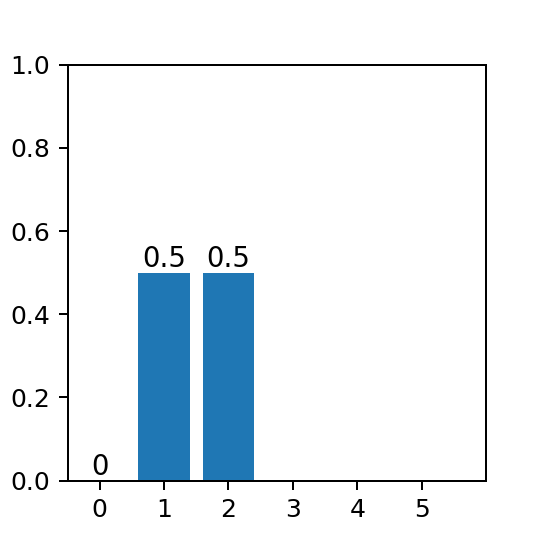
\includegraphics[width=\textwidth]{figures/ex_backlog.png}
        \caption{$f_{\mathcal{C}_1}$}\label{}
    \end{subfigure}
    \quad
    \begin{subfigure}[c]{0.3\textwidth}
        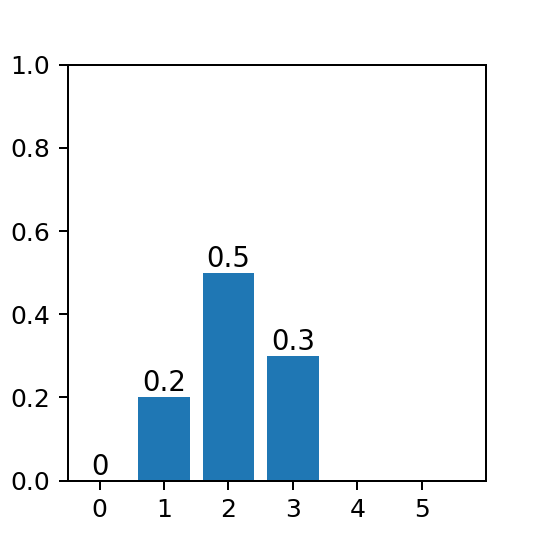
\includegraphics[width=\textwidth]{figures/ex_job_pmf.png}
        \caption{$f_{\mathcal{C}_2}$}\label{}
    \end{subfigure}
    \quad
    \begin{subfigure}[c]{0.3\textwidth}
        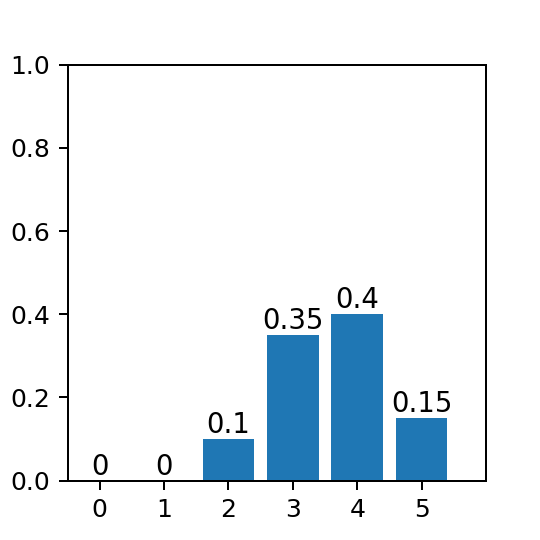
\includegraphics[width=\textwidth]{figures/ex_convolve.png}
        \caption{$\text{convolve}(f_{\mathcal{C}_1}, f_{\mathcal{C}_2})$}\label{}
    \end{subfigure}
    \caption{Convolving two job PMFs}\label{fig:convolve}
\end{figure}

\subsubsection{Shrinking}
Looking at our jobs from above, we now may want to find out how much time is still left for execution at $t = 3$. For worst-case purposes the calculation is simple:
\begin{equation*}
    C_{1+2} - (t - t_0) = 5 - 3 = 2
\end{equation*}

Again considering the probability distribution of pending workload, the analogous operation is called \textit{shrinking}:
\begin{equation*}
    \text{shrink}(f_{\mathcal{C}_{1+2}}, (t - t_0)) = [0.45, 0.4, 0.15]
\end{equation*}
As one might recognize from this example, shrinking is performed by "shifting" the distribution by some amount of time to the left and accumulating all values shifted to or past 0 in the origin, see \cref{fig:shrink}.

\begin{figure}[h]
\centering
    \begin{subfigure}[c]{0.4\textwidth}
        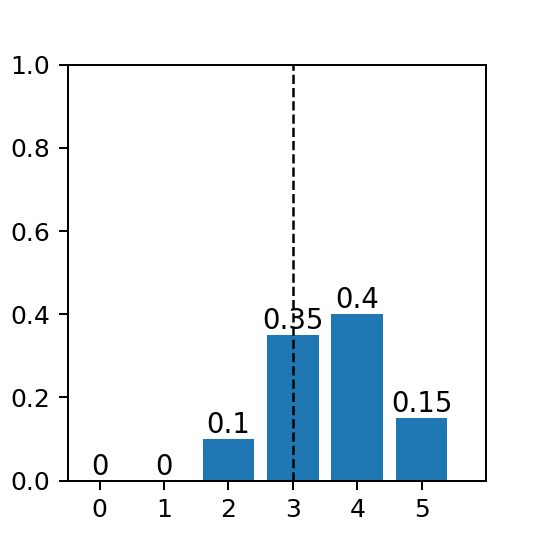
\includegraphics[width=\textwidth]{figures/ex_convolve_line.png}
        \caption{$f_{\mathcal{C}_{1+2}}$}\label{}
    \end{subfigure}
    \quad
    \begin{subfigure}[c]{0.4\textwidth}
        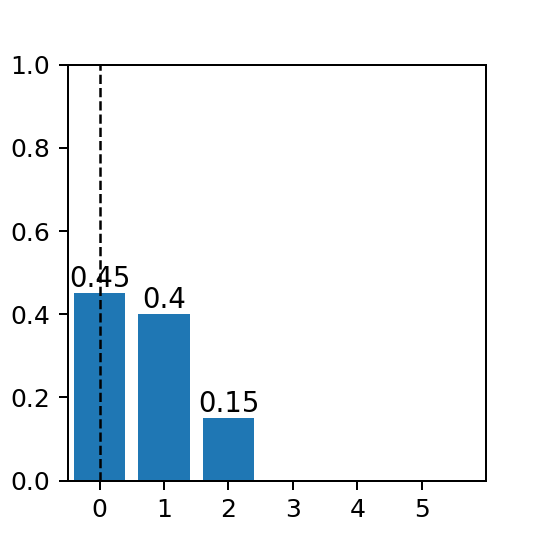
\includegraphics[width=\textwidth]{figures/ex_shrink.png}
        \caption{$\text{shrink}(f_{\mathcal{C}_{1+2}}, 3)$}\label{}
    \end{subfigure}
    \caption{Shrinking by 3}\label{fig:shrink}
\end{figure}
\subsection{Backlog Computation}
\label{subsec:backlog-comp}
To make guarantees on job DMPs for a specific schedule, we face the issue of potentially infinitely many job releases. To address this, we have to make use of the fact that these releases follow a repeating pattern, defined as the task set's \textbf{hyperperiod}. The length of one such hyperperiod, denoted by $T$, is equal to the least common multiple over all task periods $T_i$ in the task set. One can easily validate that job releases will always repeat after $T$ time units, independent of all other parameters.

A job's response time depends on three factors, namely \textit{a)} its own execution time; \textit{b)} the jobs preempting it and their execution times; and \textit{c)} the pending workload $\mathcal{W}_{\lambda_{i,j}}^{P_{i,j}}$ related to jobs of priority $P_{i,j}$ and higher at the time of release $\lambda_{i,j}$. While the pattern of job releases, i.e. \textit{a)} and \textit{b)}, is repeated for every hyperperiod, the pending workload at each job release accumulates from one hyperperiod to the next, and is thus non-repeating. I will refer to this workload as the job-level \textbf{backlog}, denoted $\mathcal{V}_{i,j} = \mathcal{W}_{\lambda_{i,j}}^{P_{i,j}}$. It can be obtained from the $P_{i,j}$-level initial system backlog $\mathcal{B}_k^{P_{i,j}} = \mathcal{W}_{kT}^{P_{i,j}}$ at the beginning of each hyperperiod. Note that these initial backlogs are non-repeating random variables themselves; however, it can be shown that their distributions converge to a stationary \textbf{steady-state} $\mathcal{B}_\infty^P$ for any $P$, as long as the total average system utilization is less than 100\% \cite{diaz2003stochastic}. It is this steady-state that finally allows us to find job response time distributions without having to consider the infinite sequence of releases. Since the convergence happens to be monotonically increasing, we can also be sure to cover the worst-case by assuming steady-state backlog distribution.

\subsubsection{Steady-state system backlog}
\label{subsubsec:stdy-st-blog}
Given the backlog distribution at the start of any hyperperiod, the initial backlog distribution of the following hyperperiod can always be computed for any priority level $P$ as follows:
\begin{enumerate}
    \item Start with backlog $\mathcal{B}_k^P$.
    \item Shrink the current backlog up to the next job release. Only jobs with priority $P$ or higher are taken into account.
    \item Convolve the current backlog with this job's execution time PMF.
    \item Repeat steps 2 and 3 until there are no more (eligible) job releases in this hyperperiod.
    \item Shrink the current backlog to the end of this hyperperiod.
\end{enumerate}

Backlog $\mathcal{B}_{k+1}^P$ thus only depends on the preceding backlog $\mathcal{B}_k^P$, and the stochastic process $\{\mathcal{B}_0^P, \mathcal{B}_1^P, ..., \mathcal{B}_k^P, ...\}$ can be proven to be a Markov chain \cite{diaz2003stochastic}. This gives us a way to find an exact solution for the steady-state in theory, but it is not well-suited for computation due to many ill-conditioned equations and prohibitively large computational complexity. For this reason I deemed the analytical solution beyond the scope of this framework; refer again to \cite{diaz2003stochastic} for more information. I will instead follow the iterative approach described there as well:
\begin{enumerate}
    \item Start with the empty backlog $\mathcal{B}_0^P$, i.e. $\mathbb{P}[\mathcal{B}_0^P = 0] = 1$.
    \item From backlog $\mathcal{B}_k^P$, compute backlog $\mathcal{B}_{k+1}^P$ with the method described above.
    \item Repeat step 2 until the approximation is "close enough".
\end{enumerate}
The condition "close enough" could be given if the square distance between iterations drops below a certain $\epsilon$, for example. \Cref{fig:backlogs} illustrates this process for three different systems. It also shows the influence of a system's utilization values: If both maximum and average utilization are less than 1, the iteration will converge (to an empty backlog if all phases are zero) after only one hyperperiod (\cref{subfig:backlogs0}). If average utilization is less than 1, but maximum utilization exceeds 1, pending work can start to accumulate at the end of each hyperperiod, but its distribution will still converge (\cref{subfig:backlogs1}). Only with average utilization above 100\%, the distribution of pending workload grows infinitely with each hyperperiod (\cref{subfig:backlogs2}).

While this method is preferred for our purposes, I would still like to mention its drawbacks: \textit{a)} Since the backlog is monotonically increasing, the approximation will always be slightly more optimistic than the exact solution, rendering this method invalid for upper-bound analysis (although the square difference decreases exponentially), and \textit{b)} finding the right value for $\epsilon$ is still an open question, as the speed of convergence depends on task set utilization, and the number of iterations needed is not known beforehand.

\begin{figure}[p]
\centering
    \begin{subfigure}[c]{\textwidth}
        \centering
        \begin{tabular}{@{}c|ll@{}}
            \toprule
            & \multicolumn{2}{c}{Utilization} \\
            System & maximum ($U(LO)$) & average ($U(avg)$) \\ 
            \midrule
            (b) & 0.833 & 0.604 \\
            (c) & 1.208 & 0.979 \\
            (d) & 1.5 & 1.125
        \end{tabular}
        \caption{Utilization values for the example systems}\label{subfig:backlogs-systems}
    \end{subfigure}
    
    \begin{subfigure}[c]{0.3\textwidth}
        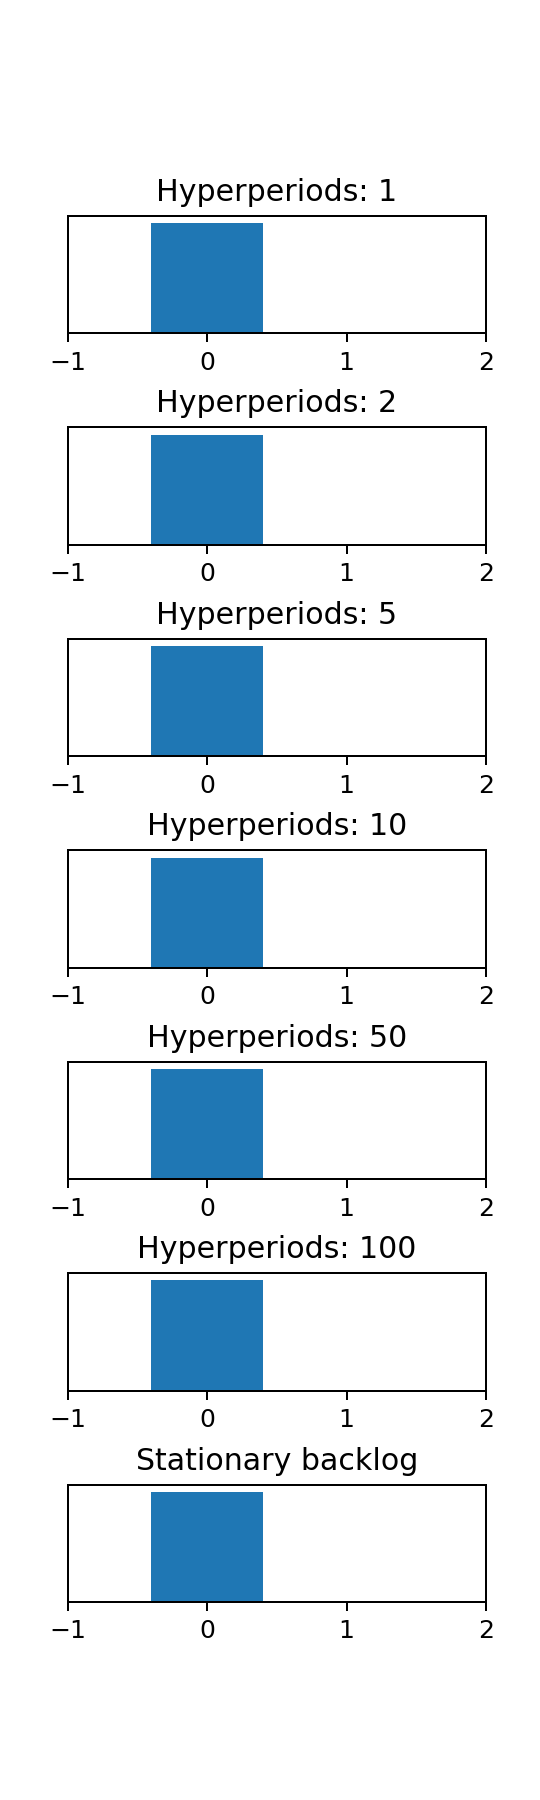
\includegraphics[width=\textwidth]{figures/ex_backlogs0.png}
        \caption{$U(LO) < 1$}\label{subfig:backlogs0}
    \end{subfigure}
    \quad
    \begin{subfigure}[c]{0.3\textwidth}
        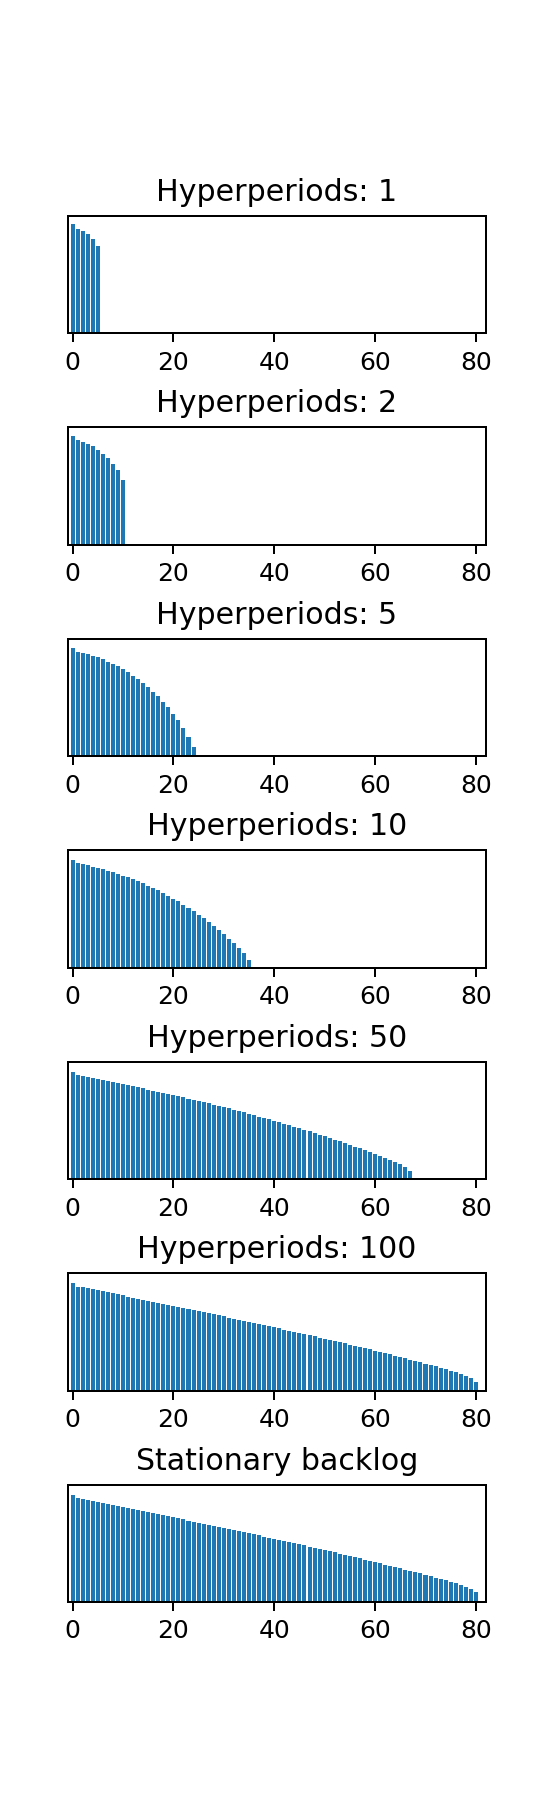
\includegraphics[width=\textwidth]{figures/ex_backlogs1.png}
        \caption{$U(avg) < 1 < U(LO)$}\label{subfig:backlogs1}
    \end{subfigure}
    \quad
    \begin{subfigure}[c]{0.3\textwidth}
        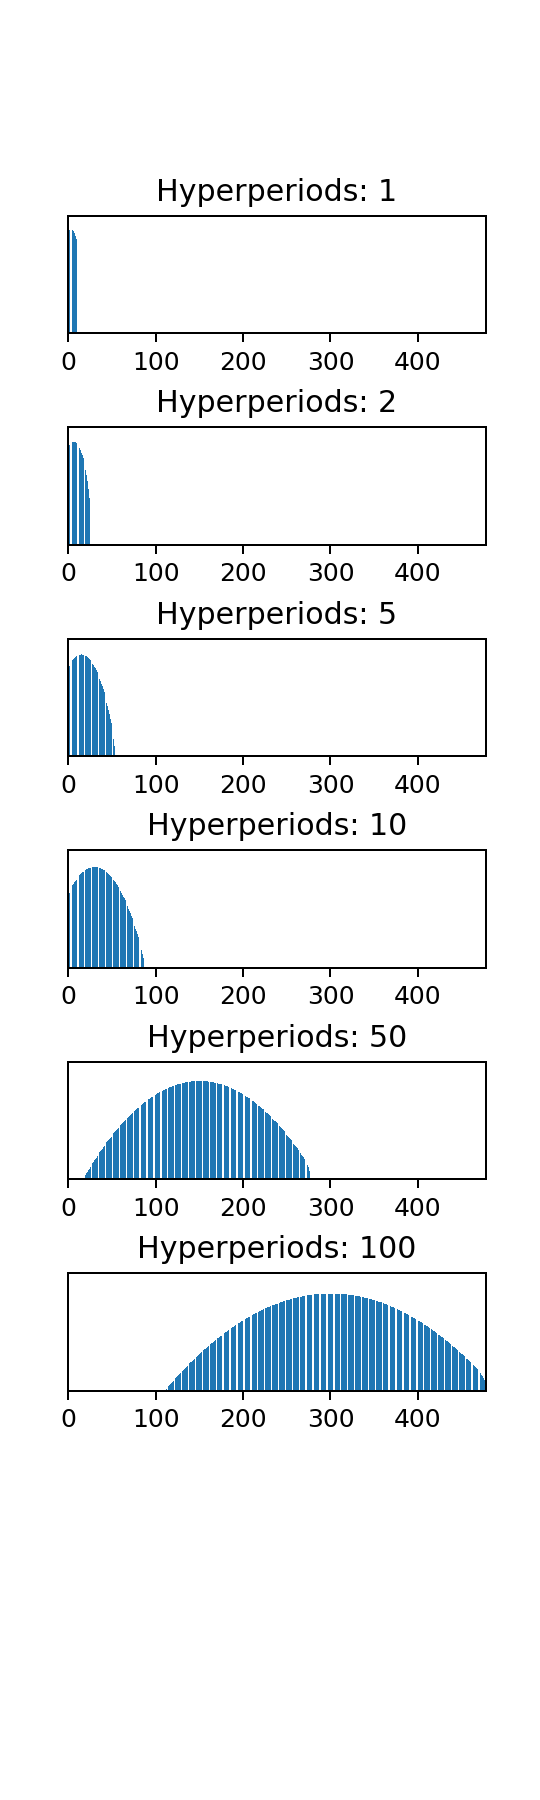
\includegraphics[width=\textwidth]{figures/ex_backlogs2.png}
        \caption{$U(avg) > 1$}\label{subfig:backlogs2}
    \end{subfigure}
    \caption{Evolution of backlog PMFs in the example systems, y-axis log-scaled}\label{fig:backlogs}
\end{figure}

\subsubsection{Job-level backlogs}
Now, to obtain the job-level backlog for any job $\Gamma_{i,j}$ in a fixed-priority system is fairly simple: Start from steady-state initial system backlog $\mathcal{B}_\infty^{P_{i,j}}$, then work your way towards the release of $\Gamma_{i,j}$, while repeatedly shrinking the intermediate distribution and convolving it with all jobs with equal or higher priority and released before $\Gamma_{i,j}$. There exists a similar method for dynamic-priority scheduled systems \cite{diaz2002stochastic}, but its implementation is left for future work.

\subsection{Response time analysis (RTA)}
\label{subsec:job-rta}
With the job-level backlog we are now ready to find any job's response time PMF $f_{\mathcal{R}_{i,j}}(\cdot)$. For job $\Gamma_{i,j}$ we first convolve the job-level backlog PMF $f_{\mathcal{V}_{i,j}}(\cdot)$ and its execution time PMF $f_{\mathcal{C}_{i}}(\cdot)$. After that, we have to take all jobs that could preempt $\Gamma_{i,j}$ (i.e. higher-priority jobs released with or after $\Gamma_{i,j}$), denoted by $\Gamma'_1, \Gamma'_2, ..., \Gamma'_k, ...$, into consideration step-by-step. At each step $k$, the new intermediate PMF is calculated by performing the following \textbf{split-convolve-merge} operation:
\begin{enumerate}
    \item \textit{Split} the intermediate PMF from step $k-1$ into a tail part ranging from the release instant of $\Gamma'_k$, $\lambda^\prime_k$, to $\infty$ and the remaining head part.
    \begin{figure}[h]
    \centering
        \begin{subfigure}[c]{0.3\textwidth}
            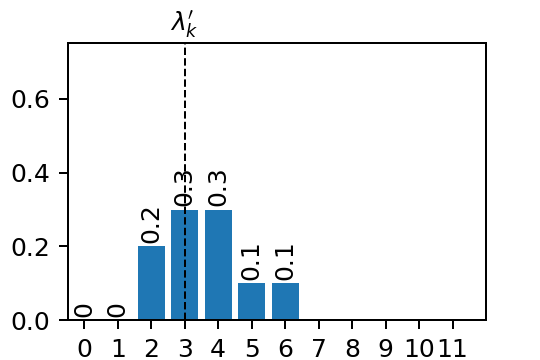
\includegraphics[width=\textwidth]{figures/ex_split_1a.png}
            \caption{before splitting}
        \end{subfigure}
        \begin{subfigure}[c]{0.3\textwidth}
            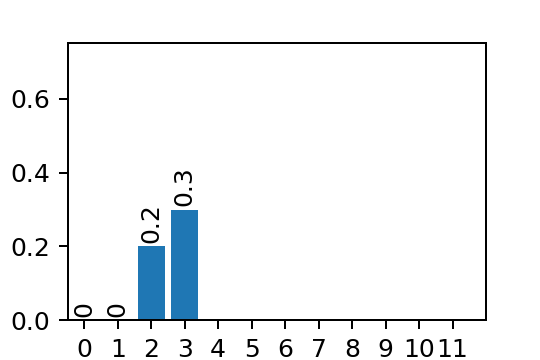
\includegraphics[width=\textwidth]{figures/ex_split_1b.png}
            \caption{head part}
        \end{subfigure}
        \begin{subfigure}[c]{0.3\textwidth}
            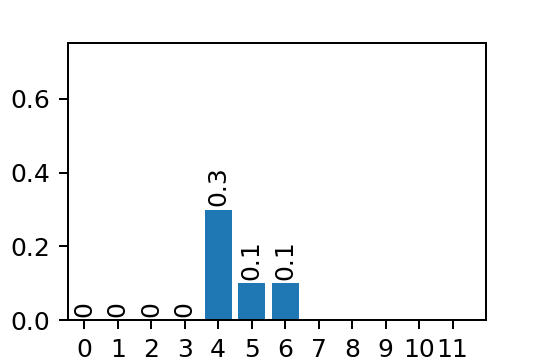
\includegraphics[width=\textwidth]{figures/ex_split_1c.png}
            \caption{tail part}
        \end{subfigure}
        \caption{Split for $\lambda^\prime_k = 3$}
    \end{figure}
    \item \textit{Convolve} only the tail part with the execution time PMF $f_{\mathcal{C}^\prime_k}(\cdot)$ of $\Gamma'_k$ since it has no influence on the execution of $\Gamma_{i,j}$ if the latter has already completed before $\lambda^\prime_k$.
    \begin{figure}[h]
    \centering
        \begin{subfigure}[c]{0.3\textwidth}
            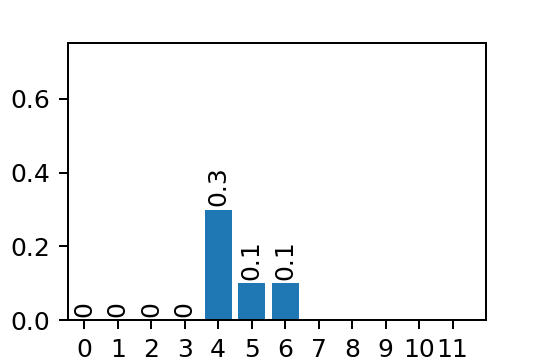
\includegraphics[width=\textwidth]{figures/ex_split_2a.png}
            \caption{tail part}
        \end{subfigure}
        \begin{subfigure}[c]{0.3\textwidth}
            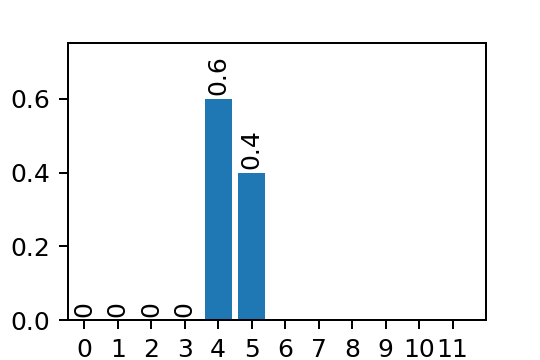
\includegraphics[width=\textwidth]{figures/ex_split_2b.png}
            \caption{$f_{\mathcal{C}^\prime_k}(\cdot)$}
        \end{subfigure}
        \begin{subfigure}[c]{0.3\textwidth}
            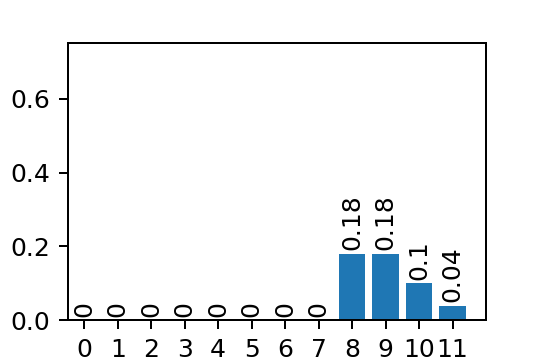
\includegraphics[width=\textwidth]{figures/ex_split_2c.png}
            \caption{after convolving}
        \end{subfigure}
        \caption{Convolve}
    \end{figure}
    \item \textit{Merge} the two parts back together to obtain the new intermediate PMF.
    \begin{figure}[h]
    \centering
        \begin{subfigure}[c]{0.3\textwidth}
            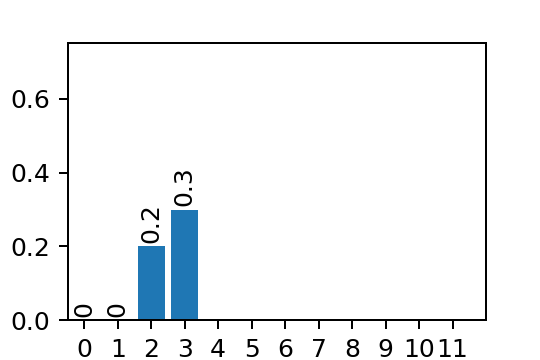
\includegraphics[width=\textwidth]{figures/ex_split_3a.png}
            \caption{head part}
        \end{subfigure}
        \begin{subfigure}[c]{0.3\textwidth}
            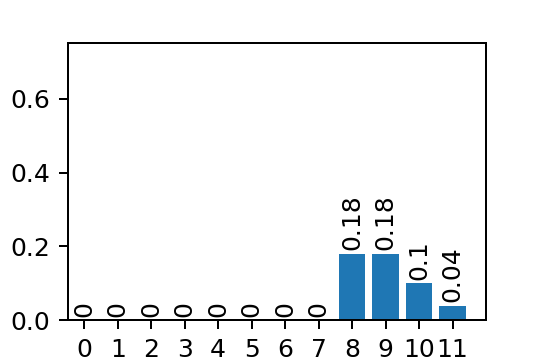
\includegraphics[width=\textwidth]{figures/ex_split_3b.png}
            \caption{tail part}
        \end{subfigure}
        \begin{subfigure}[c]{0.3\textwidth}
            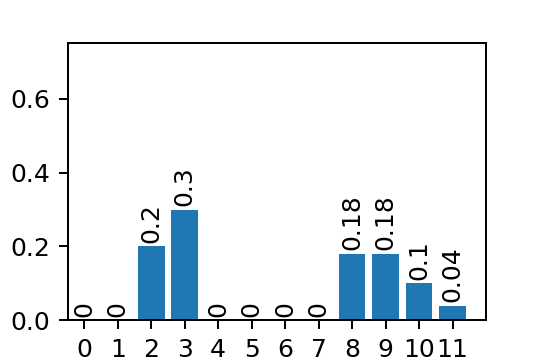
\includegraphics[width=\textwidth]{figures/ex_split_3c.png}
            \caption{after merging}
        \end{subfigure}
        \caption{Merge}
    \end{figure}
\end{enumerate}

Note that, although in theory the list of interrupting jobs $\Gamma'_k$ could be infinitely long, in practice we only have to consider interruptions up to the deadline $D_i$ of $\Gamma_{i,j}$ if we are interested in deadline miss probabilities, as $\mathbb{P}[\mathcal{R}_{i,j} > D_i] = 1 - \mathbb{P}[\mathcal{R}_{i,j} \leq D_i]$.

\subsection{Probabilistic Schedulability Schemes}
\label{subsec:prob-schemes}
We can now build on our deterministic schemes using the principles introduced in \crefrange{subsec:basic-ops}{subsec:job-rta}. Systems are typically rated based on their DMP per hour. The new schemes thus will revolve around the idea that all tasks have to offer a DMP below a certain threshold to be deemed schedulable. For this, we will, for every task $\tau_i$, look at all jobs $\Gamma_{i,j}$ in one hyperperiod and calculate the probability that at least one of them misses their deadline as follows:
\begin{equation*}
    \textit{DMP per hyperperiod} = 1 - \mathbb{P}[\textit{no deadline miss}] = 1 - \prod_j \mathbb{P}[\mathcal{R}_{i,j} \leq D_i]
\end{equation*}
First I present a probabilistic variant of our static mixed criticality scheme. Then I propose a stochastic extension to AMC.
\subsubsection{pSMC}
This scheme is similar to SMC as again there is no notion of different system criticality modes used here. For every task $\tau_i$, its corresponding job DMPs are calculated using the methods described above. As shown, they can then be used to find the probability of $\tau_i$ missing a deadline in one hyperperiod. By using different thresholds, this offers the possibility to judge tasks based on their criticality, where HI-tasks must fulfill harder requirements than LO-tasks.
\subsubsection{pAMC-BB}
Extending AMC to a probabilistic scheme can be proposed as follows: Suppose that the system's behavior after a switch to HI-mode is unknown, a "black box" (BB). We simply assume that this black box will have a fixed duration $n_{HI}$ (e.g. one full hyperperiod), after which the system is reset back to LO-mode.

This means that only the conditional PMF for LO-mode has to be considered in the analysis. There are no changes for LO-tasks, since their PMFs only range up to $C_i(LO)$ anyways. For HI-tasks, however, we first calculate their probability of \textit{not} triggering a mode switch per job release:
\begin{equation*}
    \mathbb{P}[\mathcal{C}_i \leq C_i(LO)] = \sum_{x = 0}^{C_i(LO)} f_{\mathcal{C}_{i}}(x) \qquad \mbox{if } \chi_i = HI
\end{equation*}
We then crop their PMF at $C_i(LO)$ and normalize it, defining the conditional PMF "given the system stays in LO-mode":
\begin{equation*}
    f_{\mathcal{C}_{i}}^{LO}(x) = \begin{cases} \frac{1}{\mathbb{P}[\mathcal{C}_i \leq C_i(LO)]} \cdot f_{\mathcal{C}_{i}}(x) &\quad \mbox{if } x \in [0, C_i(LO)] \\ 0 &\quad \mbox{otherwise} \end{cases}
\end{equation*}.

Now, we calculate the probability of a mode switch happening per hyperperiod over all tasks:

\begin{equation*}
    p_{switch} = 1 - \prod_i (\mathbb{P}[\mathcal{C}_i \leq C_i(LO)])^{m_i},
\end{equation*}
where $m_i = \frac{T}{T_i}$ is the number of instances of task $\tau_i$ per hyperperiod.

With $p_{switch}$ we can compare the overall times spent in LO-mode and HI-mode. The expected number of hyperperiods until a switch to HI-mode occurs amounts to 
\begin{equation*}
    n_{LO} = \frac{1}{p_{switch}},
\end{equation*}
as the sequence of hyperperiods represent Bernoulli trials with failure probability $p_{switch}$, and the probability distribution of the first $C(LO)$ overrun thus is a geometric one.

Finally, we can find an aggregate DMP for each task:
\begin{equation*}
    \phi_i = \frac{n_{LO}}{n_{LO} + n_{HI}} \cdot \phi_i^{LO} + \frac{n_{HI}}{n_{LO} + n_{HI}} \cdot \phi_i^{HI}
\end{equation*}
Here, $\phi_i^{LO}$ is the DMP in LO-mode, calculated again by applying the response time analysis method described above to both LO- and HI-tasks (the latter with the now adjusted, conditional PMF). $\phi_i^{HI}$, a task's DMP for HI-mode, on the other hand, is given by the black box and defines the penalty for a mode switch; for instance, assume it to be 1 for LO-tasks (assumed to miss all deadlines) and 0 for HI-tasks (assumed to meet all deadlines). This $\phi_i$ can now again be compared to criticality-specific thresholds to decide overall schedulability of this task set. 

Note that, in contrast to their deterministic counterparts, pAMC-BB does not subsume pSMC in general and instead tries to offer a model somewhat closer to realistic applications. Both their results greatly depend on the confidence values for $C_i(LO)$ and $C_i(HI)$ as well as the chosen acceptance thresholds. For the framework I will assume suitable values for these to be given. Finally, I would like to mention the work of Maxim et al. \cite{maxim2016probabilistic} on a different probabilistic implementation of SMC and AMC, where they focused more on manipulating the task set's execution time PMFs.


\subsection{Monte Carlo Simulation}
\label{subsec:monte-carlo-schemes}
Last but not least, another possible way of deciding on schedulability is to just simulate execution for huge numbers of hyperperiods ($\geq 10^5$). This means drawing a random sample from a task's execution time PMF every time a new job instance is released, then executing it while respecting the considered scheme's priority assignment and other special cases (e.g. mode switches in pAMC). At the end, every tasks DMP can be estimated by counting deadline misses relative to all hyperperiods. 

This method is called a \textit{Monte Carlo Simulation} and has the great benefit of being flexible and simple (no response time analysis needed at all), but its severe drawbacks are quite obvious, too: Besides being just a sampling approximation, enormous amounts of simulated hyperperiods are also needed for high resolution. For instance, with "only" $10^4$ hyperperiods, the smallest non-zero DMP a task can have is $10^{-4}$, which cannot be compared sensibly to a passing threshold of $10^{-9}$. I will return to Monte Carlo simulations for pSMC and pAMC in \cref{cha:eval} for comparison, but as a tool for analysis, their theoretical counterpart methods are generally preferred.

%%%%%%%%%%%%%%%%%%%%%%%%%%%%%%%%%%%%%%%%%%%%%%%%%%%%%%%%%%%%%%%%%%
\chapter{The Framework}
\label{cha:framework}
In this chapter, I provide details to the actual implementation of the framework. In \cref{sec:framework-overview} the necessary software requirements are listed and a general top-level overview is given. The rest of the chapter then describes the individual components, each related to a separate source file. Note that I focus mainly on the questions of \textit{how} and \textit{why} here; for further information on the exact APIs and their usage, see the source files and the corresponding docstrings directly.

\section{Overview}
\label{sec:framework-overview}
For the implementation of the framework, I chose \textbf{Python 3}, based on its many advantages:
\begin{itemize}
    \item Its object-orientation facilitates an understandable, direct implementation of many components of the proposed system model.
    \item It proves to be very efficient at handling large amounts of data such as thousands of probability distributions.
    \item An abundance of different tool kits enables the broad spectrum of topics covered, ranging from scientific computation to visualization.
    \item Python is generally seen as clean and easy to read, and enjoys great popularity in the academic as well as the industrial community, making it accessible to many people.
\end{itemize}
The entire source code is available online\footnote{\url{https://github.com/luca-stalder/bsc-thesis}}. The Python version used is 3.6.0. A number of additional packages are necessary, as listed in \cref{py-packages}. One often used Python distribution covering all required tools is the \textit{Anaconda Distribution}\footnote{\url{https://www.continuum.io/downloads}} for Python 3, a toolbox commonly used for data science related work. The latest version at the time of writing is \textit{Anaconda 4.4.0}.

\begin{table}[ht]
    \centering
    \caption{Python packages used}
    \label{py-packages}
    \begin{tabular}{@{}ll@{}}
        \toprule
        Package & Version \\
        \midrule
        matplotlib & 2.0.2 \\
        numpy & 1.12.1 \\
        scipy & 0.19.0 \\
    \end{tabular}
\end{table}

\section{Library Module: \texttt{lib.py}}
This file contains basic object definitions as well as common functions used throughout the framework.
\subsection{Container Classes}
\texttt{Task} is our basic task object. It contains all necessary attributes as fields. In the entire framework, I assume period, deadline, $C(LO)$, and $C(HI)$ to be integer values. A task's execution time PMF is stored as an array. The entry on index k corresponds to the probability for an instance of this task to run for k time units:
\begin{equation*}
    \texttt{task\_i.c\_pmf[k]} == P[\mathcal{C}_i = k]
\end{equation*}


\texttt{TaskSet} then is a closed set of multiple \texttt{Task} objects. It offers multiple functions to get the different system utilization values, as well as a method to display the set's description and its visual representation. 

When initializing a new task set, a timeline of \texttt{Job} objects within one hyperperiod is built, if possible. This class will later be used to store another PMF as a vector, namely the job's response time PMF $\mathcal{R}_{i,j}$. This PMF does not necessarily have to be complete (i.e. sum up to 1), as the values up to the job's deadline are sufficient to find the jobs DMP.

\subsection{Common Functions}
\texttt{convolve\_rescale\_pmf(a, b, percentile)} implements the convolution operation described in \cref{subsec:basic-ops} as follows: The actual convolution of the two arrays is done by scipy's \texttt{convolve()}. Depending on the input size, this method derives the result either directly from the sums, or via Fast Fourier Transform, which performs faster for large input arrays. As a second step, we then drop all values past at a certain \texttt{percentile}, given as parameter, and normalize the final result so that it sums up to 1 again. This cropping is necessary, as without it, the arrays representing PMFs would grow larger and larger with repeated convolutions. It is a trade-off, but with a small cutoff percentile ($10^{-14}$) little precision is lost in this process.

\texttt{shrink()} represents the shrink operation introduced in \cref{subsec:basic-ops}, and \texttt{split\_convolve\_merge()} is an implementation of the algorithm with the same name described in \cref{subsec:job-rta}. Both implementations are trivial.

\subsection{Probability Distribution Classes}
\label{subsec:prob-dist-cls}
The classes defined here are used by the generation module to define execution time PMFs for newly generated tasks. Further distributions can be defined, as long as they implement \textit{a)} \texttt{from\_percentile(x\_lo, p\_lo, x\_hi, p\_hi)}, a constructor method creating a distribution object with \texttt{x\_lo} and \texttt{x\_hi} at percentile values \texttt{p\_lo} and \texttt{p\_hi}, respectively; and \textit{b)} \texttt{discrete\_pmf(cutoff)}, a function returning a discretized approximation of its PMF as an array. The \texttt{cutoff} parameter defines again the upper limit, after which the approximation shall be cropped, to avoid unbounded arrays. See the following section for more on the individual distributions included here.

\section{Task Set Synthesis: \texttt{synthesis.py}}
Although evaluating different ways of generating synthetic task sets is not the main focus of this framework, the generation itself still plays a major role, as proper schedulability test analysis would not be possible without. This module deals with our need to generate such task sets. To do so, I have split up the process into two distinct problems: First, generate a set of tasks with just their deterministic parameters such as period and $C(LO/HI)$ values (\cref{subsec:synth-param}); then fit a probability distribution to each task, such that its $C(LO/HI)$ values lie at set percentiles (\cref{subsec:synt-dist}). Different solutions for each of these sub-problems should be interchangeable. See \cref{subsec:synth-ex} for examples for some possible combinations.

\subsection{Task Set Parameters}
\label{subsec:synth-param}

\subsubsection{SimpleGen}
Many papers on the subject of mixed-criticality systems such as \cite{baruah2011response} use an enhanced version of the \textbf{UUniFast} algorithm \cite{bini2005measuring}, which was designed to find utilization values adding up to a certain sum in general, and not with mixed-criticality in mind. Following their example, I implemented the synthesis method I call \texttt{simplegen()} as follows:
\begin{enumerate}
    \item For a given system utilization, generate a set of \texttt{n\_tasks} LO-mode task utilizations using UUnifast. Since UUnifast was designed with system utilizations of at most 1 in mind, call UUnifast multiple times with fractions of the desired \texttt{u\_lo}, if necessary.
    \item For each task, uniformly draw a period out of the set \texttt{periods = [5, 10, 20, 25, 50, 100]}. Although these values may be chosen a bit arbitrary, they ensure a manageable hyperperiod of length 100, while still providing enough spread between the smallest and largest values. Multiply the period with \texttt{time\_granularity} to reduce discretization error from rounding values.
    \item Assign each task either HI- or LO-criticality, based on \texttt{cp}, the chance of being HI-critical.
    \item Define \texttt{c\_lo} based on the product of task utilization and period; round up the result to avoid \texttt{c\_lo == 0}.
    \item For HI-critical tasks, define \texttt{c\_hi} as a constant multiple \texttt{cf} of \texttt{c\_lo}; again round up to avoid \texttt{c\_lo == c\_hi}.
    \item If desired (\texttt{implicit\_deadlines == False}), uniformly draw a random deadline from the range $[\texttt{cf*c\_lo}, \texttt{period}]$, else set the deadline equal to the period.
\end{enumerate}

\subsubsection{MC-FairGen}
Another algorithm was recently developed by Ramanathan et al. \cite{ramanathan2016evaluation} and poses a more sophisticated approach to generate mixed-criticality task sets. It respects several \textit{fairness properties} defined there, introduces parameters for minimum and maximum per-task utilization, and also supports multi-core systems. Although single core systems are considered here, we can still exploit this feature to generate task sets with utilizations above 100\%. My implementation \texttt{mc\_fairgen()} generally follows their proposal while making a few adjustments:
\begin{itemize}
    \item Execution times, periods, and deadlines are again rounded to integers.
    \item Periods are chosen out of the set \texttt{[5, 10, 20, 25, 50, 100]} instead of the entire uniform distribution from 5 to 100. This is again to keep hyperperiods small.
    \item I again discretize all final values and introduce the \texttt{time\_granularity} parameter as a multiplier to reduce rounding errors.
\end{itemize}

\subsection{Execution Time Distributions}
\label{subsec:synt-dist}

\subsubsection{Exponential Exceedance Functions}
To now add execution time PMFs to these tasks, we can use \texttt{synth\_c\_pmf()} with the \texttt{ExpExceedDist} class as parameter. Maxim et al. \cite{maxim2016probabilistic} suggested generating such a distribution based on the 1-CDF (Complementary Cumulative Distribution Function or \textbf{exceedance function}) of the task's execution time PMF. On this exceedance function, the following requirements are imposed:
\begin{itemize}
    \item It is represented by a straight line on a graph with exceedance probabilities given on a log scale. For instance, this is the case for a function of the form:
    \begin{equation}
    \label{eq: 1-cdf}
        \text{1-CDF:\qquad} ex(x) = a \cdot \text{exp}(b \cdot x)
    \end{equation}
    \item $C(LO)$ and $C(HI)$ values lie on fixed exceedance probabilities $ex_{LO}$ and $ex_{HI}$.
    \item It is only defined in the range $[C(min), C(HI)]$, with $ex(C(min)) \overset{!}{=} 1$. If the task is LO-critical, $C(HI)$ is substitued with $CP \cdot C(LO)$, where $CP$ is again a constant criticality factor (e.g. $CP = 1.5$).
\end{itemize}
Solving the first two constraints as well as $ex(C(min)) = 1$ yields the following expressions for $a$, $b$, and $C(min)$:
\begin{equation}
\label{eq:param-expr}
    a = \frac{ex_{LO}}{\text{exp}(b \cdot C(LO))}, \quad b = \frac{\text{ln}(ex_{HI}) - \text{ln}(ex_{LO})}{C(HI) - C(LO)}, \quad C(min) = - \frac{\text{ln}(a)}{b}
\end{equation}

Furthermore, we can derive the probability density function from \cref{eq: 1-cdf}:
\begin{equation}
    \text{PDF}: \qquad f(x) = - a \cdot b \cdot \text{exp}(b \cdot x), \qquad \text{for $x \geq C(min)$}
\end{equation}

Using the expressions from \cref{eq:param-expr}, a distribution can thus be fitted to each task with the constructor method \texttt{from\_percentile()}. The \texttt{ExpExceedDist} object's \texttt{discrete\_pmf()} then returns a discrete approximation (\cref{subsec:prob-dist-cls}).

\subsubsection{Weibull Distributions}
The Weibull distribution can be another well-suited tool to generate execution time PMFs. This heavy-tailed distribution is defined by the density function
\begin{equation}
    PDF\footnote{Since these functions are used as execution times, we only consider the positive part of them here.} : \qquad f(x) = \frac{k}{\beta} \cdot \left( \frac{x}{\beta} \right)^{k - 1} \cdot \text{exp}\left(-\left(\frac{x}{\beta}\right)^k\right).
\end{equation}
The class \texttt{WeibullDist} can also be passed to \texttt{synth\_c\_pmf} and sets up instances of this distribution as follows:
\begin{itemize}
    \item Uniformly draw a value between $1.5$ and $3.0$ for its shape parameter k. The shape of the distribution's density function depends on k; only values $k > 1$ yield the bell-like curves I deemed characteristic for task execution time distributions (\cref{fig:task-set-mc-fairgen}).
    \item Next, from its cumulative distribution function
    \begin{equation}
        CDF : \qquad F(x) = 1 - \text{exp}\left(-\left(\frac{x}{\beta}\right)^k\right)
    \end{equation}
     and the given values for $C(LO)$ and its percentile $p_{LO}$, derive the following expression for its scale parameter $\beta$:
    \begin{equation}
        \beta = \frac{C(LO)}{\left(-\text{ln}(1 - p_{LO})\right)^\frac{1}{k}}
    \end{equation}
    \item Finally, initialize the object with \texttt{k} and \texttt{beta} and compute the discrete approximation again by calling its \texttt{discrete\_pmf()} function (\cref{subsec:prob-dist-cls}).
\end{itemize}

\subsection{Examples}
\label{subsec:synth-ex}
\Cref{fig:task-set-simplegen} shows a first example task set which was generated using \texttt{simplegen()} and the \texttt{ExpExceedDist} class. Parameters were chosen as follows: \texttt{u\_lo=0.8}, \texttt{cf=1.5}, \texttt{cp=0.5}, \texttt{n\_tasks=10}, \texttt{implicit\_deadlines=False}, and percentile values \texttt{c\_lo\_percent=1-1e-5} and \texttt{c\_hi\_percent=1-1e-9}.

\begin{figure}[p]
    \centering
    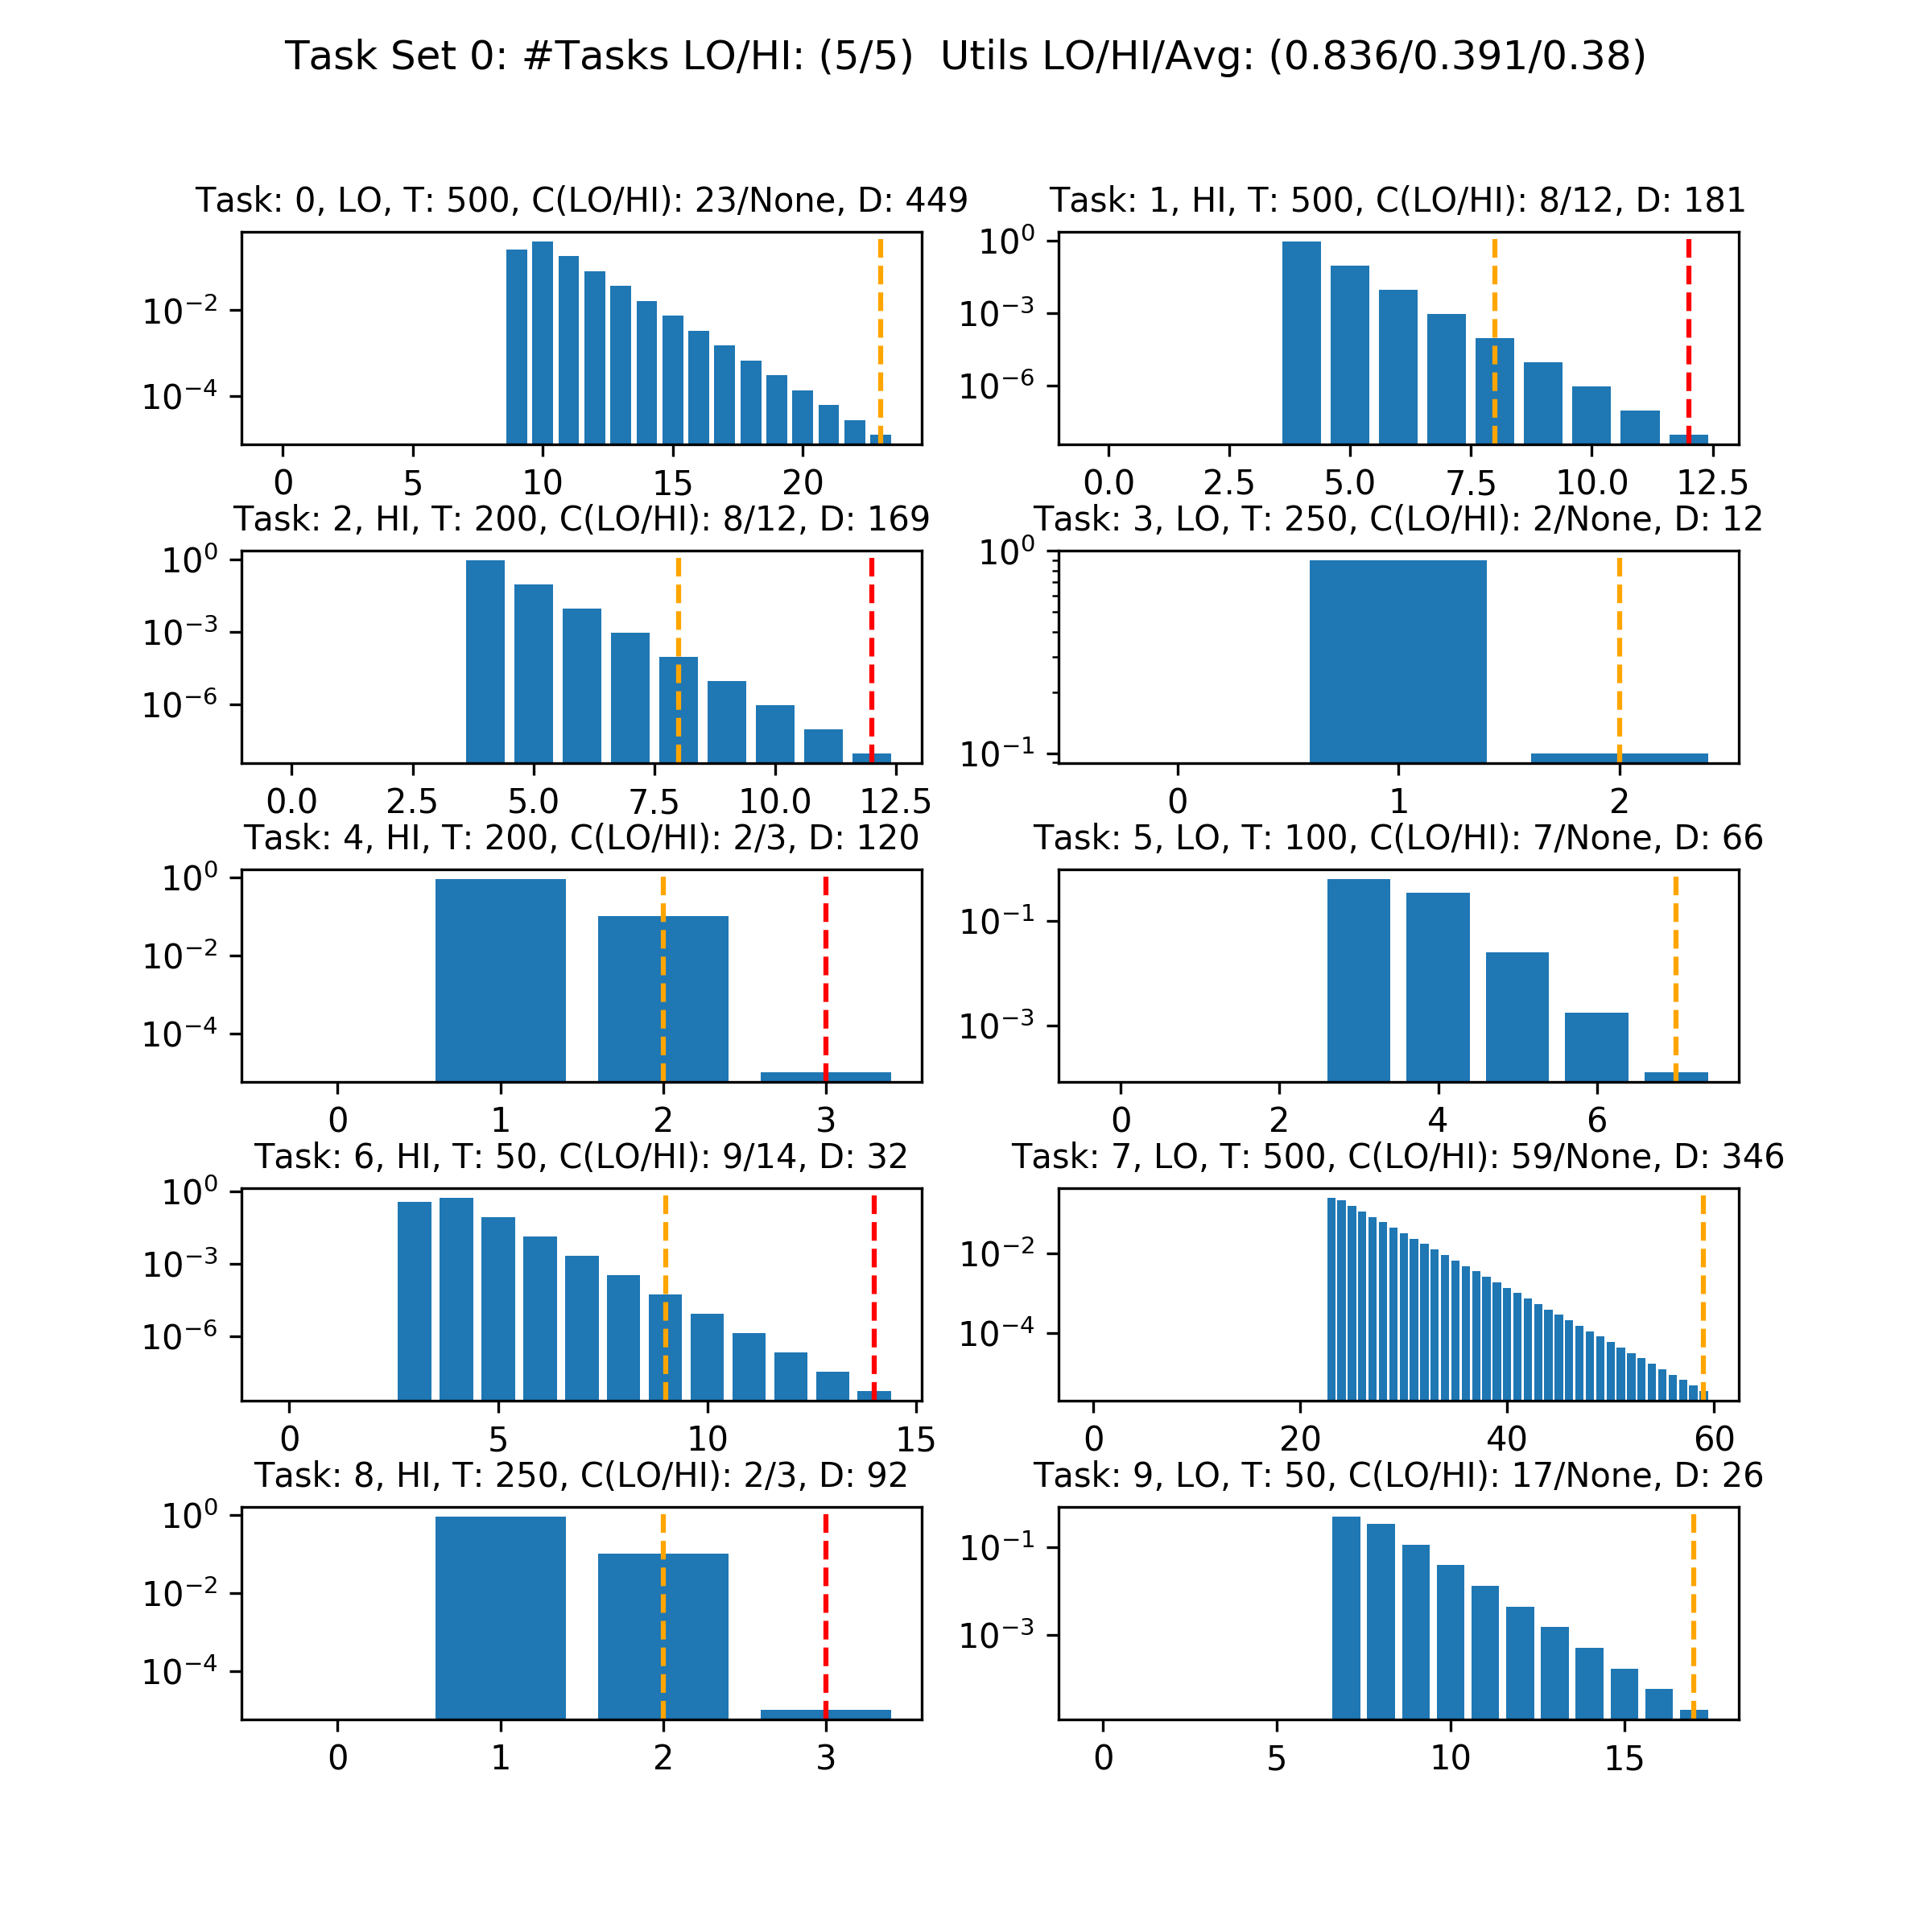
\includegraphics[width=\textwidth]{figures/ex_simplegen.png}
    \caption{UUniFast with ExpExceedDist, log-scaled y-axis, orange and red lines corresponding to $C(LO)$ and $C(HI)$ values}\label{fig:task-set-simplegen}
\end{figure}

Another example is shown in \Cref{fig:task-set-mc-fairgen}, representing \texttt{mc\_fairgen()} in combination with Weibull distributions. Parameters were chosen as follows: \texttt{u\_lo=0.8}, \texttt{implicit\_deadlines=False}, and the percentile values \texttt{c\_lo\_percent=1-1e-5} and \texttt{c\_hi\_percent=1-1e-9}.

\begin{figure}[p]
    \centering
    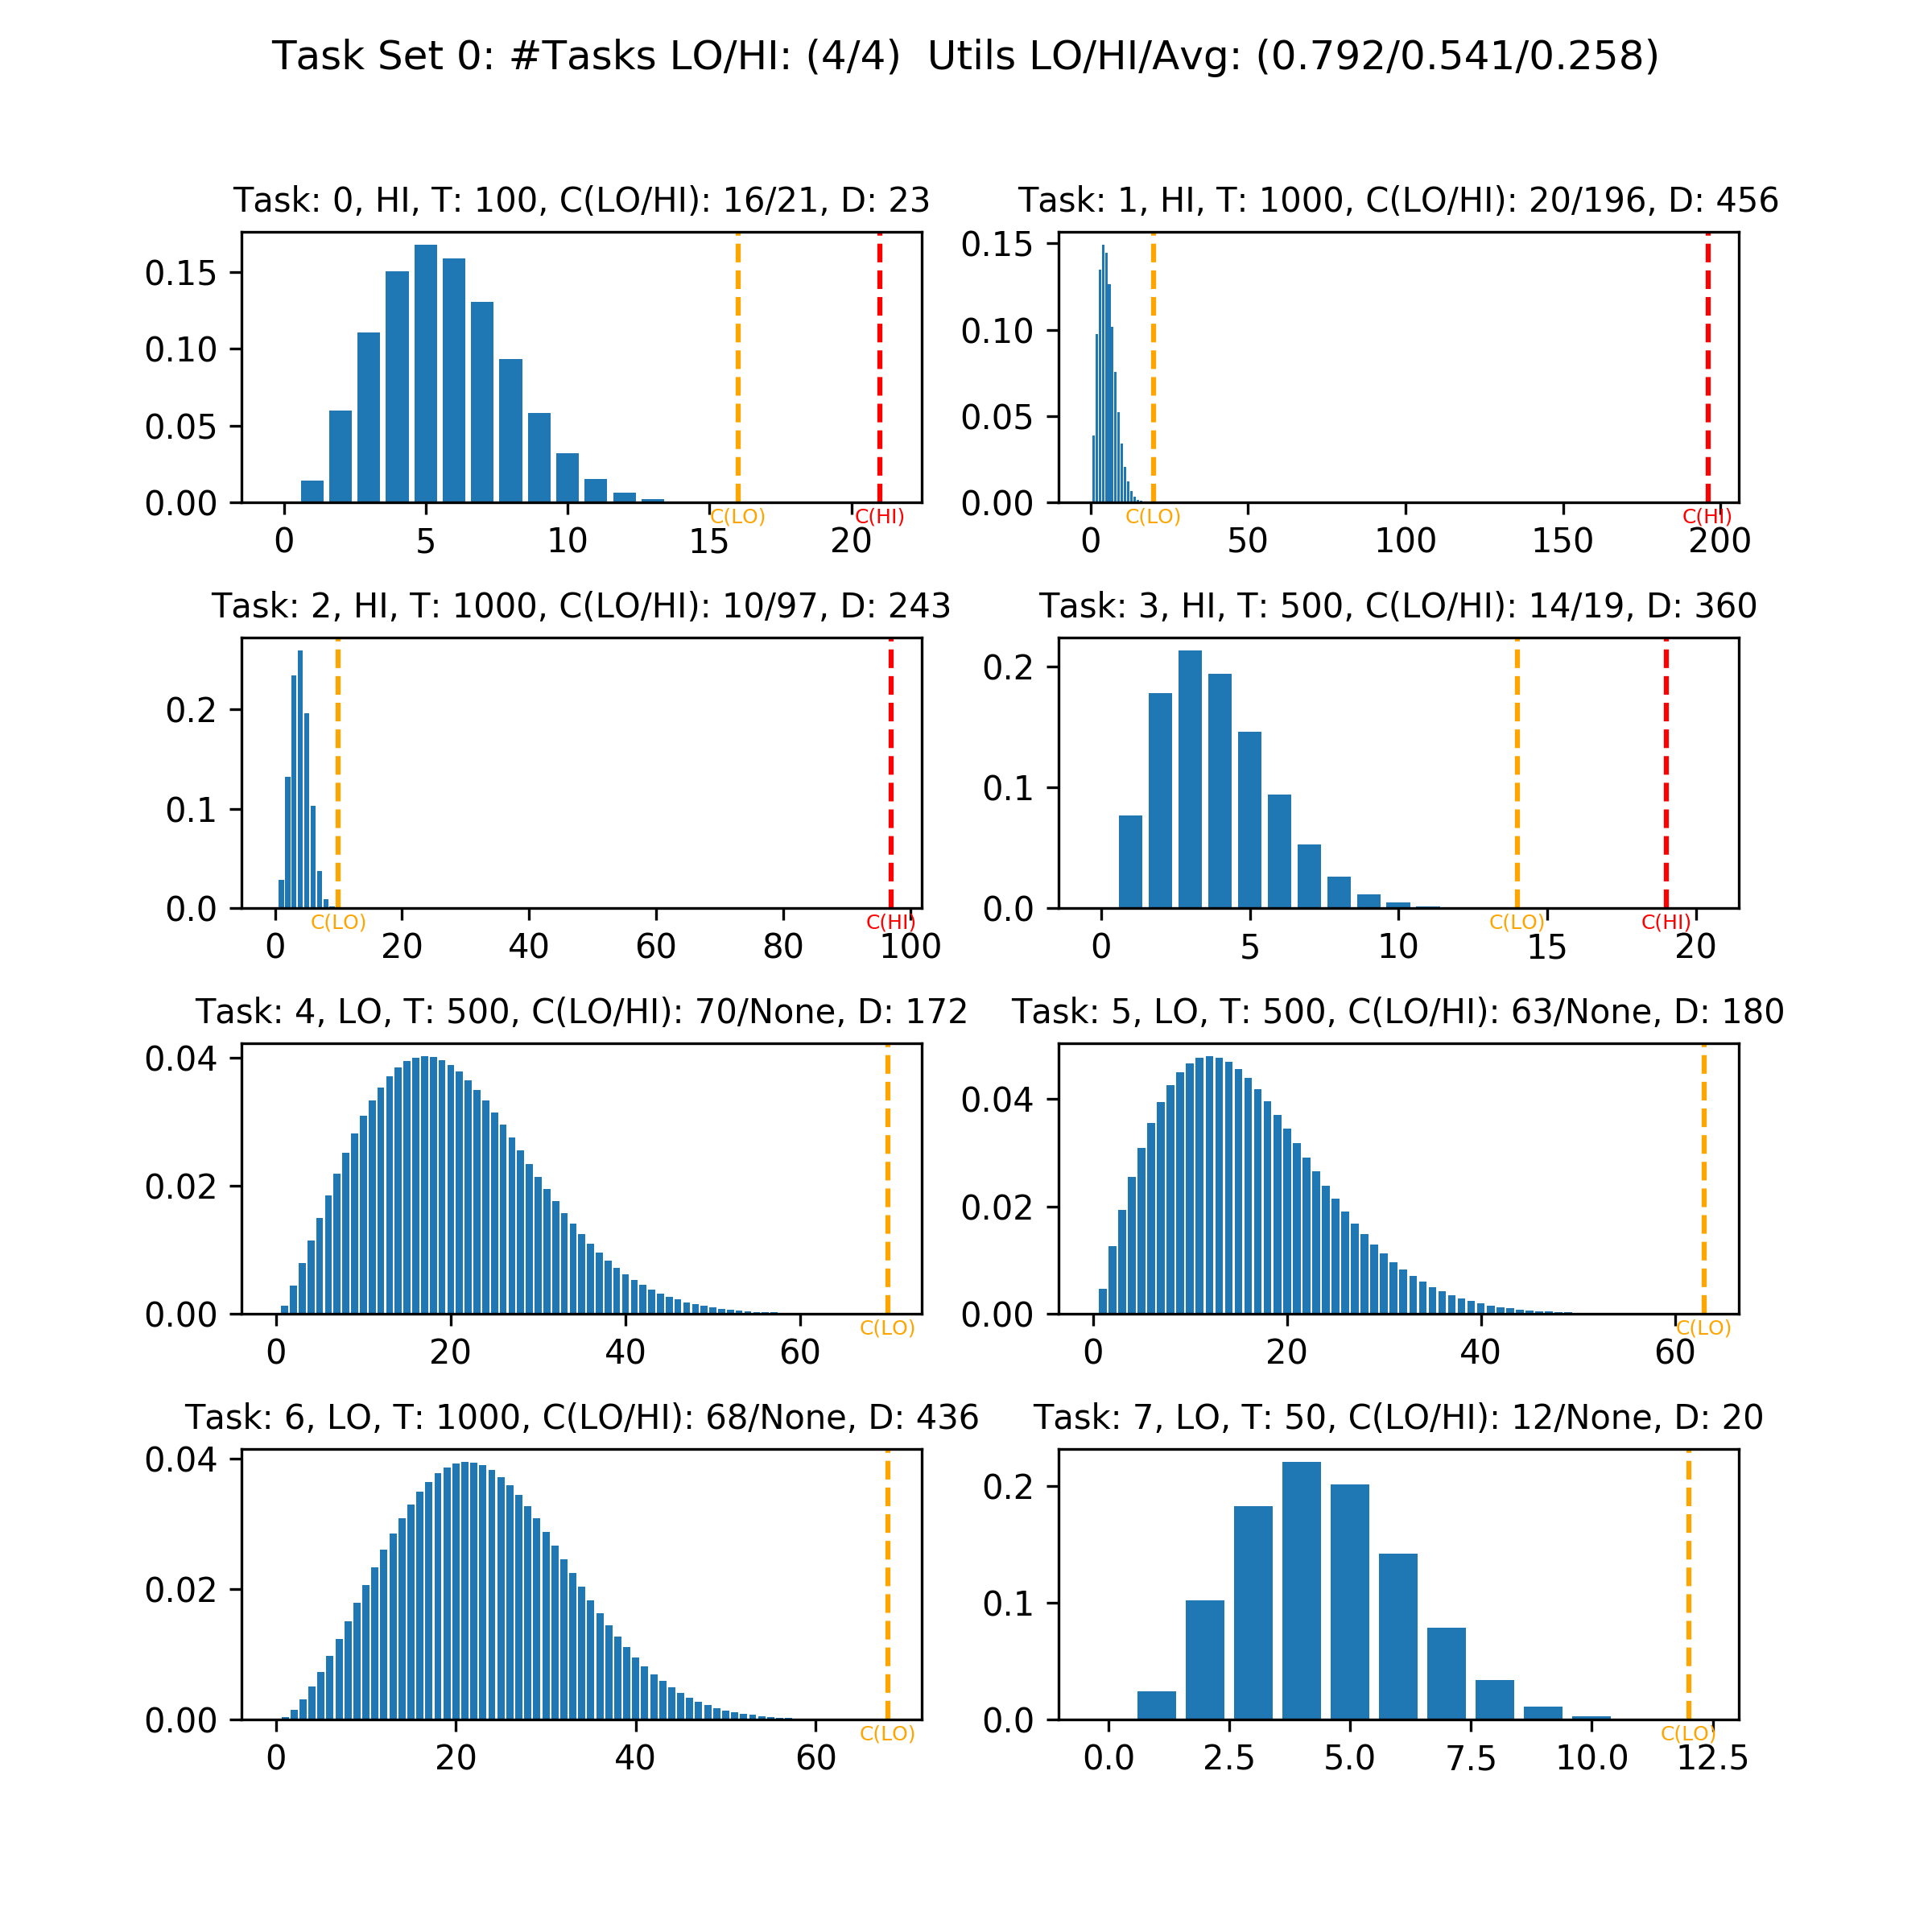
\includegraphics[width=\textwidth]{figures/ex_mc_fairgen.png}
    \caption{MC-FairGen with Weibull Distributions, linear y-scale, orange and red lines corresponding to $C(LO)$ and $C(HI)$ values}\label{fig:task-set-mc-fairgen}
\end{figure}

\newpage
\section{Schedulability Tests: \texttt{analysis.py}}
This module revolves around response time and schedulability analysis, i.e. the concepts introduced in \cref{sec:sys-model-det-ana} and \cref{sec:sys-model-prob-ana}.
\subsection{Response Time Analysis Tools}
The \texttt{BacklogSim} object is the main container for iterative convolving and shrinking of backlogs. It is initialized with a given \texttt{task\_set} and a set \texttt{p\_level}. Its \texttt{step(dt, mode)} function will simulate a \texttt{dt} unit time step in the system, including newly reached job releases and the convolution of their execution time, shrinking the current backlog on the way to the next release, as well as wrapping around if the end of the current hyperperiod is reached in the process. This object is used both for finding stationary backlog and individual job-level response time PMFs. For visualization, see the animation module in \cref{sec:anim-mod}.

\texttt{stationary\_backlog\_iter()} is used to determine a task set's steady-state backlog at a desired \texttt{p\_level}. It first checks the sets average utilization; if above 100\%, then the backlog will not converge. Otherwise it instantiates a \texttt{BacklogSim} object and performs simulation steps of one full hyperperiod at a time. Every backlog at time \texttt{t == 0} is compared with the last, measuring the quadratic difference between the two arrays. As soon as this difference drops below the threshold \texttt{epsilon}, or \texttt{max\_iter} iterations have been performed, the loop is stopped and the result is returned.

\texttt{rta\_fp()} calculates all job-level response time PMFs in a fixed-priority scheduled task set. First, for each priority level the steady-state backlog is calculated using \texttt{stationary\_backlog\_iter()}. Using these initial backlogs, every job's individual backlog is found by iterative convolution and shrinking up to its release. Finally, the job response time distribution is obtained using the split-convolve-merge operation described in \cref{sec:sys-model-prob-ana}. This distribution is attached as \texttt{response} to every \texttt{Job} object in the task set.
\subsection{Deterministic Schedulability Tests}
The methods \texttt{d\_smc}, \texttt{d\_amc}, and \texttt{d\_edf\_vd} defined in this section implement deterministic analysis tools for the schemes listed in \cref{sec:sys-model-det-ana}. They all take a \texttt{TaskSet} object as an input, and return \texttt{True} iff the task set is schedulable using the corresponding scheme. For \texttt{d\_smc} and \texttt{d\_amc}, tasks need to have fixed priorities assigned (see \texttt{generation} module).
\subsection{Probabilistic Schedulability Tests}
\texttt{p\_smc} and \texttt{p\_amc\_bb} are the implementation of \cref{subsec:prob-schemes}. Both take threshold parameters in addition to a task set, and use \texttt{rta\_fp()} to find each job's response time PMF. \texttt{p\_smc} directly compares the resulting task per-hyperperiod deadline miss probabilities to the thresholds \texttt{thresh\_lo} and \texttt{thresh\_hi}, depending on the task's criticality. \texttt{p\_amc\_bb} first finds the probability of a mode switch, adjusts the HI-tasks' execution time PMFs as described, and then applies \texttt{rta\_fp()} to these. Finally, the combined LO- and HI-mode DMP is evaluated. Both method return \texttt{True} iff all tasks pass the threshold.

\subsection{Monte Carlo Schedulability Tests}
Finally, these methods represent the Monte Carlo Simulations described in \cref{subsec:monte-carlo-schemes}: \texttt{p\_smc\_monte\_carlo} and \texttt{p\_amc\_bb\_monte\_carlo}. While their API is very similar, their implementations differ fundamentally from their analytic counterparts. They will actually run the task set for a number of hyperperiods (\texttt{nhyperperiods}), drawing an execution time value at each job release and counting every hyperperiod a deadline miss occurred for each task. If at one point this number grows too big, the simulation is stopped and \texttt{False} is returned. With \texttt{p\_amc\_bb}, execution times are also monitored; if a mode switch occurs, the simulation clears its backlog and skips \texttt{hi\_mode\_duration} hyperperiods ahead, counting the skipped hyperperiods as failed for all LO-tasks. Since the resolution of these resulting deadline miss probabilities depends on \texttt{nhyperperiods}, and increasing this number becomes very expensive quickly, these methods generally have to be run with more generous thresholds to yield meaningful results.

\section{Evaluation: \texttt{evaluation.py}}
\label{sec:eval-mod}
This module contains a collection of scripts applying the various synthesis and analysis methods defined in the other parts of the framework. Scripts in the synthesis section will generate task sets for different utilization values, defined by the \texttt{utils} parameter. Different schedulability test schemes are then performed in the next section of the module. All task sets as well as the resulting schedulability rates for every scheme are stored on disk, using the \texttt{pickle} module, such that they may be reused at a later time. Finally, the resulting schedulability rates can be plotted against their corresponding task set's \texttt{u\_lo} value. The resulting plots will be discussed in greater detail in \cref{cha:eval}.

A note about performance: Stochastic schedulability tests generally come with high computational cost, mainly stemming from steady-state backlog computation. To alleviate this, all schedulability test scripts use the Python library \texttt{multiprocessing} to spawn a pool of worker processes. Input task sets are then distributed evenly across these processes. The reason for multiple processes rather than threads is the Python Global Interpreter Lock (GIL)\footnote{https://wiki.python.org/moin/GlobalInterpreterLock}, which prohibits parallel execution of multiple threads. See \cref{sec:performance} for a list of speedups this implementation achieves.

\section{Energy Module: \texttt{energy.py}}
\label{sec:energy-mod}
This module is an implementation for \cref{cha:energy}. Note that all probability mass functions are again stored as arrays, i.e. the value at index \texttt{i} stands for the probability of energy and/or time equalling to $i$. The main function will produce \cref{fig:energy}.

\section{Animation: \texttt{backlog\_animation.py}}
\label{sec:anim-mod}
This module offers a comprehensive demonstration for the iterative application of convolution and shrinking during steady-state backlog analysis, making use of the \texttt{animation} object contained in \texttt{matplotlib}. The example task set is generated at the top of the module; this can also be changed to other synthesis methods.

%%%%%%%%%%%%%%%%%%%%%%%%%%%%%%%%%%%%%%%%%%%%%%%%%%%%%%%%%%%%%%%%%%
\chapter{Energy Uncertainty}
\label{cha:energy}
In this chapter, I want to show that parts of the framework, especially the components manipulating PMFs, can be applied to other topics with minimal adjustments as well. For this purpose, we leave the world of mixed-criticality task sets and turn to scheduling when available energy is uncertain for a moment. First, I introduce the basic system model and basic operations, then look at an implementation thereof, and finally show some small examples of running these.

\section{System Model}
There are many different system models containing energy harvesting, but for this example let us consider the case of a single-core \textbf{transient system}. The first component of such a system is the energy management unit (EMU), collecting at the beginning of each discrete unit time interval a discrete amount of energy, determined by a random variable with the PMF $h(x)$, from an energy harvester. The EMU stores this energy in a small buffer with capacity $B$ and provides it to the processor (CPU) in the form of energy bursts of size $B$ whenever the buffer reaches full charge. $B$ is assumed to be orders of magnitude smaller than the power dissipation of any task, i.e. job response time depends primarily on its energy consumption, and not on execution time. We also define $(\cdot)^{*n}$ the operation of convolving a PMF $n$ with itself.

Since the amount of collected energy per time unit is a random variable, so is the inter-arrival time of subsequent energy bursts; we denote its PMF with $i(x)$. The corresponding cumulative distribution function is 
\begin{equation}
    I(y) = \sum_{x \geq B} h(x)^{*y}
\end{equation}
In words, $I(y)$ yields the probability that it will take \textit{at most} $y$ time units to completely fill the buffer, causing the next energy burst. The PMF \begin{equation}
    i(y) = I(y) - I(y - 1)
\end{equation}
then yields the probability that it will take \textit{exactly} $y$ time units for the next burst, giving us the desired inter-arrival time PMF.

Finally, let job $\Gamma$ have an execution time of $C$ and a power dissipation of $P$ per time unit. The response time PMF $f_\mathcal{R}(\cdot)$ of $\Gamma$ can then be computed as:
\begin{equation}
    f_\mathcal{R}(x) = i(x)^{* \ceil[\big]{\frac{C \cdot P}{B}}} \otimes \delta_C(l)\footnote{$\delta_C(x)$ denotes the discrete delta function, equal to 1 for $x = C$, and 0 otherwise.}
\end{equation}
\begin{equation*}
    \text{where } l = \begin{cases} B / P & \quad \text{if } (C \cdot P) \text{ mod } B = 0\\
    \frac{(C \cdot P) \text{ mod } B}{P} & \quad \text{otherwise}
\end{cases}
\end{equation*}

\section{Examples}
Running the \texttt{energy} module lets us examine a few examples, shown in \cref{fig:energy}.

\begin{figure}[ht]
    
    \centering
    \begin{subfigure}[b]{0.45\textwidth}
        \caption{}
        \label{subfig:energy1}
        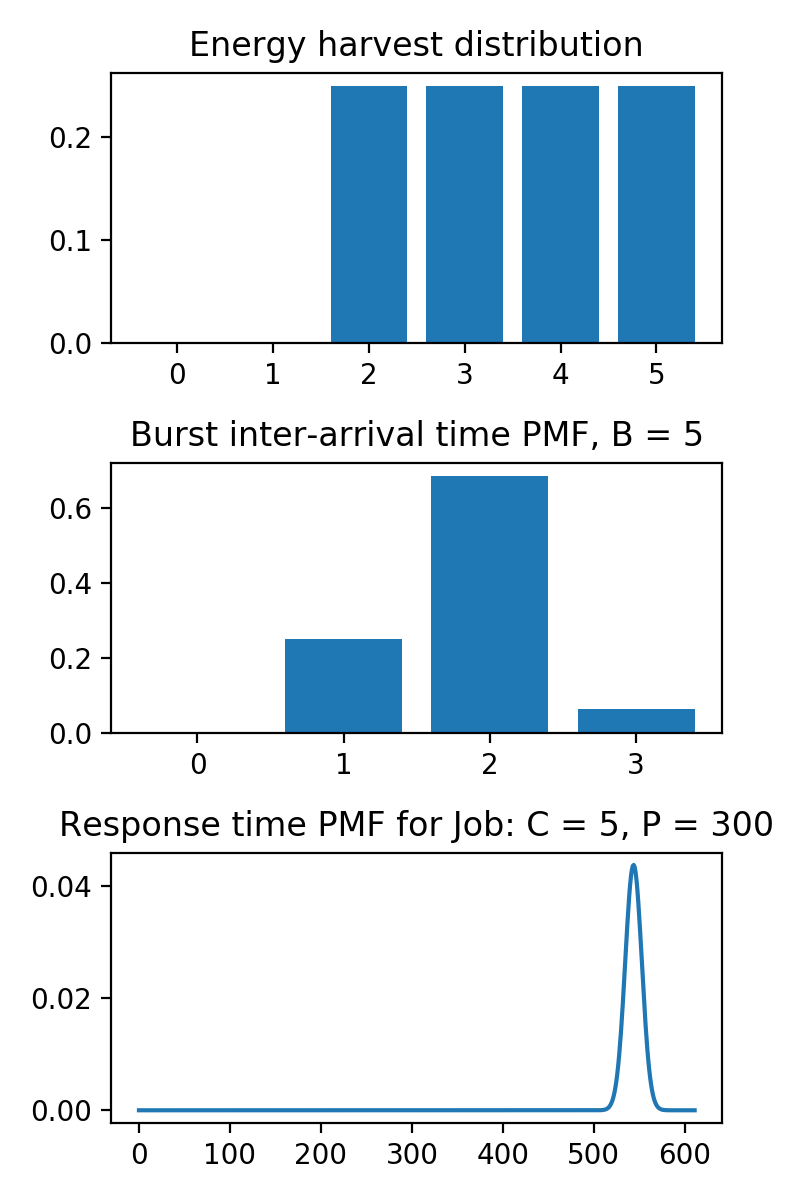
\includegraphics[width=\textwidth]{figures/energy1.png}
    \end{subfigure}
    ~
    \begin{subfigure}[b]{0.45\textwidth}
        \caption{}
        \label{subfig:energy2}
        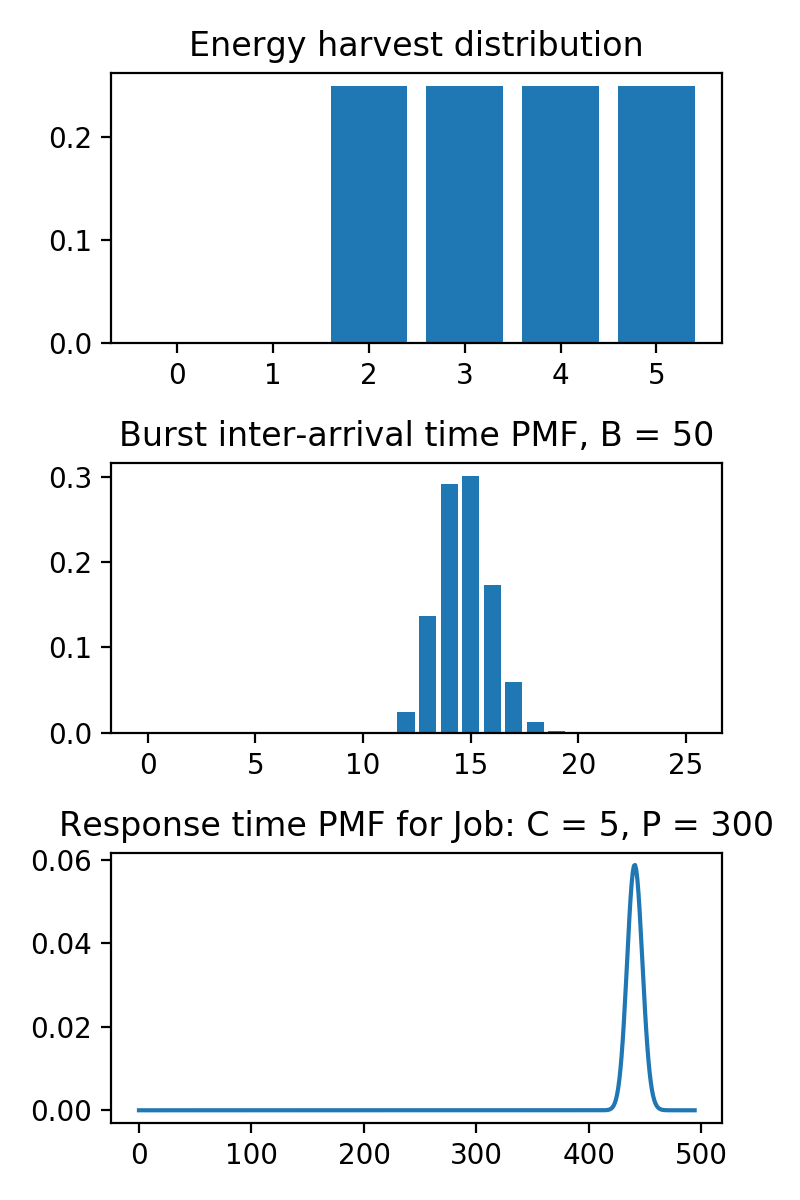
\includegraphics[width=\textwidth]{figures/energy2.png}
    \end{subfigure}
    \newline
    \newline
    \begin{subfigure}[b]{0.45\textwidth}
        \caption{}
        \label{subfig:energy3}
        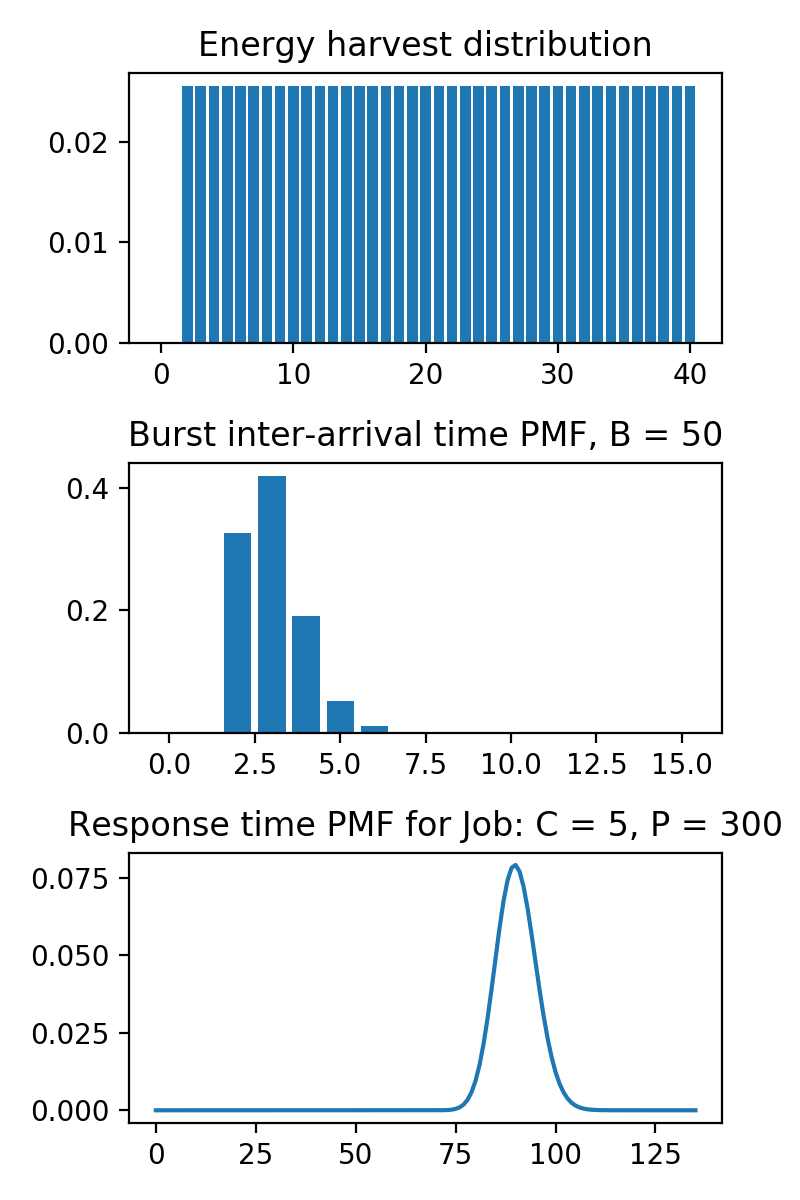
\includegraphics[width=\textwidth]{figures/energy3.png}
    \end{subfigure}
    ~
    \begin{subfigure}[b]{0.45\textwidth}
        \caption{}
        \label{subfig:energy4}
        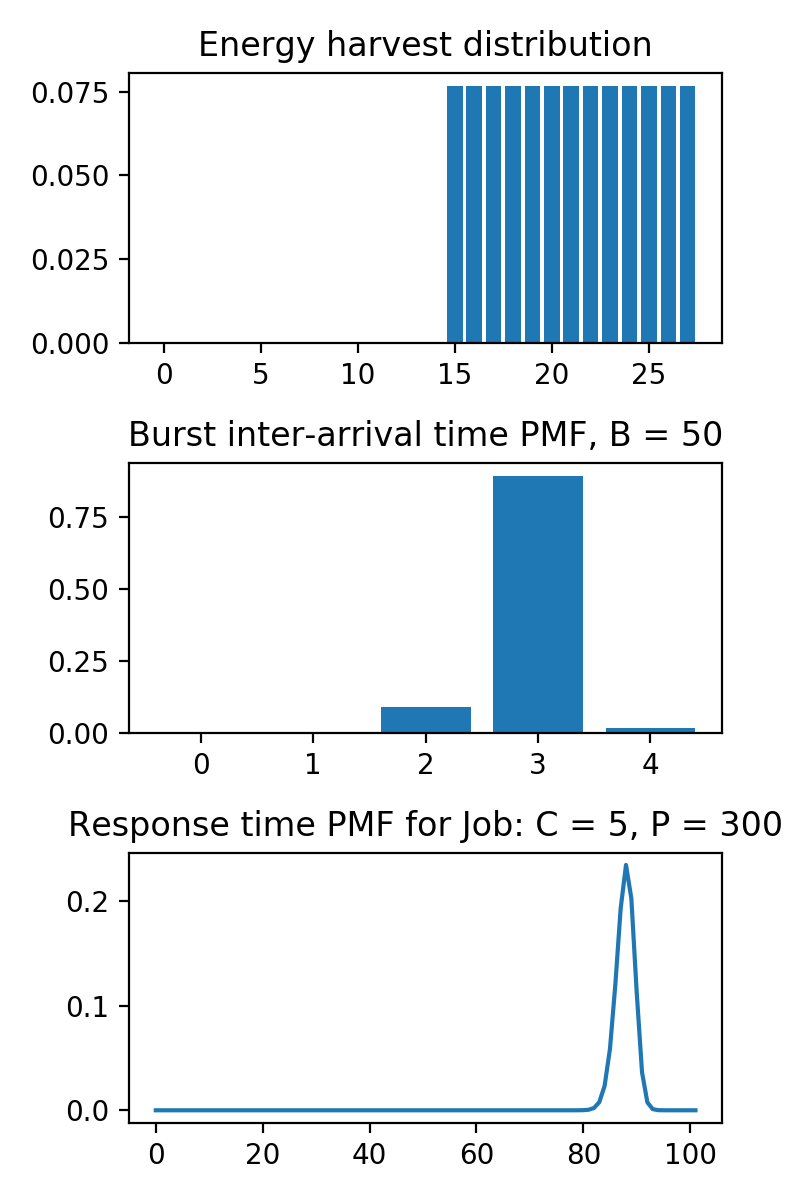
\includegraphics[width=\textwidth]{figures/energy4.png}
    \end{subfigure}
    \caption{Different transient systems}
    \label{fig:energy}
\end{figure}

Every subfigure is generated from a different input, and consists of three plots, to be interpreted as follows: The top plot shows the distribution PMF for energy collected per time unit, with energy on the x- and probability on the y-axis. The center plot shows the distribution PMF for time in between energy bursts, with time on the x- and probability on the y-axis. The bottom plot finally shows the job response time distribution's PMF, with response time on the x- and again probability on the y-axis.

The difference between \cref{subfig:energy1} and \cref{subfig:energy2} lies in $B$, the size of the system's energy buffer and bursts: Increasing $B$ from 5 to 50 improves the job's response time by roughly 100 time units in our example. This demonstrates the fact that all harvested energy exceeding the buffer's capacity "spills over" and is lost in this system model; a larger buffer makes this effect happen less frequently.

Meanwhile, \cref{subfig:energy3} and \cref{subfig:energy4} demonstrate the influence of a more reliable energy source: Although both energy harvesters provide the same amount of energy on average, the one in \cref{subfig:energy4} does this over a narrower range, resulting in a narrower range for burst inter-arrival time and job response time as well.


%%%%%%%%%%%%%%%%%%%%%%%%%%%%%%%%%%%%%%%%%%%%%%%%%%%%%%%%%%%%%%%%%%
\chapter{Evaluation}
\label{cha:eval}
In this chapter I finally put all introduced concepts together and evaluate the visualized results. In \cref{sec:eval-schemes} I compare different schemes for schedulability testing. Afterwards, in \cref{sec:performance}, I talk about some measurements on framework performance.

\section{Comparison of Test Schemes}
\label{sec:eval-schemes}

\subsection{Deterministic vs. Stochastic Test Schemes}
\subsubsection{Visualization}
\Cref{fig:eval-schemes} displays the resulting plots after running the schemes presented for two different synthesis methods. We can now compare the different schedulability tests while making some observations about the framework's capabilities and limitations at the same time. For both plots, 1000 task sets were generated and assessed per data point. The x- and y-axes represent the synthesis input parameter \texttt{u\_lo} and the percentage of task sets that were deemed schedulable, respectively. Task sets were generated with the following methods and parameters:
\begin{itemize}
    \item \textbf{\Cref{subfig:eval-schemes-simplegen}}
    \begin{itemize}
        \item Task set parameters by \texttt{simplegen()}
        \item \texttt{cf=1.5} (factor for $C(HI)$ values)
        \item \texttt{cp=0.5} (chance for $HI$ task criticality)
        \item \texttt{n\_tasks=10}
        \item \texttt{implicit\_deadlines=False}
        \item Execution time distributions by \texttt{ExpExceedDist}
        \item \texttt{c\_lo\_percent=1-1e-5} (percentile for $C(LO)$)
        \item \texttt{c\_hi\_percent=1-1e-9} (percentile for $C(HI)$)
    \end{itemize}
    \item \textbf{\Cref{subfig:eval-schemes-fairgen}}
    \begin{itemize}
        \item \texttt{implicit\_deadlines=False}
        \item \texttt{distribution\_cls=WeibullDist}
        \item \texttt{c\_lo\_percent=1-1e-5} (percentile for $C(LO)$)
        \item \texttt{c\_hi\_percent=1-1e-9} (percentile for $C(HI)$)
    \end{itemize}
\end{itemize}
On these task sets, we now run the following schedulability testing schemes:
\begin{itemize}
    \item \textbf{dSMC} \newline See \cref{subsec:dsmc}.
    \item \textbf{dAMC} \newline See \cref{subsec:damc}.
    \item \textbf{EDF-VD} \newline See \cref{subsec:edf-vd}.
    \item \textbf{pSMC} \newline See \cref{subsec:prob-schemes}. Threshold deadline miss probabilites are chosen at $10^{-4}$ and $10^{-9}$ for LO- and HI-critical tasks, respectively.
    \item \textbf{pAMC-BB} \newline See \cref{subsec:prob-schemes}. The duration of the black box state here is assumed to be one full hyperperiod. During this time, all LO-critical tasks are assumed to miss their deadlines. Threshold DMPs are chosen at $10^{-4}$ and $10^{-9}$ for LO- and HI-critical tasks, respectively.
    \item \textbf{pAMC-BB+} \newline This is an alternative version of pAMC-BB, with the difference that the LO-task deadline misses during the black box state are ignored (i.e. $\phi_i^{HI} = 0$ for all tasks $\tau_i$). Black box duration is again one hyperperiod, and threshold deadline miss probabilites are chosen at $10^{-4}$ and $10^{-9}$ for LO- and HI-critical tasks, respectively.
\end{itemize}

\subsubsection{Interpretation}
There are a few observations to make in \cref{fig:eval-schemes}:
\begin{itemize}
    
    \item Comparing deterministic schemes to stochastic ones demonstrates the implications of pessimistic worst-case analysis inherent to deterministic schemes. Whereas their schedulability rates start to drop as the system utilization approches 100\% ($C(LO)$ values considered), their probabilistic counterparts use the additional information about execution times and continue to return positive test results well beyond that boundary.

    \item pAMC-BB exhibits a somewhat peculiar line of schedulability rates. There are multiple factors at work here: It turns out, that the assumptions we are making in \cref{subsec:prob-schemes} about the black box pose a severe penalty for switching to HI-mode; so much so, that it causes schedulability rates for lower values of $U(LO)$ to be strictly dominated by the probability of a mode switch to occur in the first place. In fact, almost all task sets in the lower $U(LO)$ ranges that were not schedulable with pAMC-BB had exclusively LO-task DMPs exceed the threshold. This also explains the constant rates for all $U(LO) \leq 1$, as mode switch probability only depends on the number of tasks and the percentile of $C(LO)$ values, but not system utilization. Only when going beyond 100\% utilization, schedulability rates decline; the instant drop there is caused by both synthesis methods doubling the number of tasks when generating $U(LO) > 1$.
    
    It is clear that the shape of this curve greatly depends on the task sets analysed. To include a version of pAMC-BB that is more comparable to other methods, pAMC-BB+ has been introduced, which, everything else remaining equal, removes the penalty for switching to HI-mode. As expected, this results in rates a bit higher than for pSMC, in a similar way the curves for their deterministic counterparts, dSMC and dAMC, lie in relation to each other.

    \item For MC-Fairgen, some task sets at 100\% utilization are still schedulable for deterministic task sets. Note that the values on the x-axis are only the inputs for the synthesis; MC-FairGen has to round $C$ values during discretization, which results in task sets sometimes ending up with $U(LO) < 100\%$. SimpleGen on the other hand rounds up, as to avoid tasks with $C(LO) = 0$.
\end{itemize}

\begin{figure}[p]
    \begin{subfigure}[c]{\textwidth}
        \makebox[\textwidth][c]{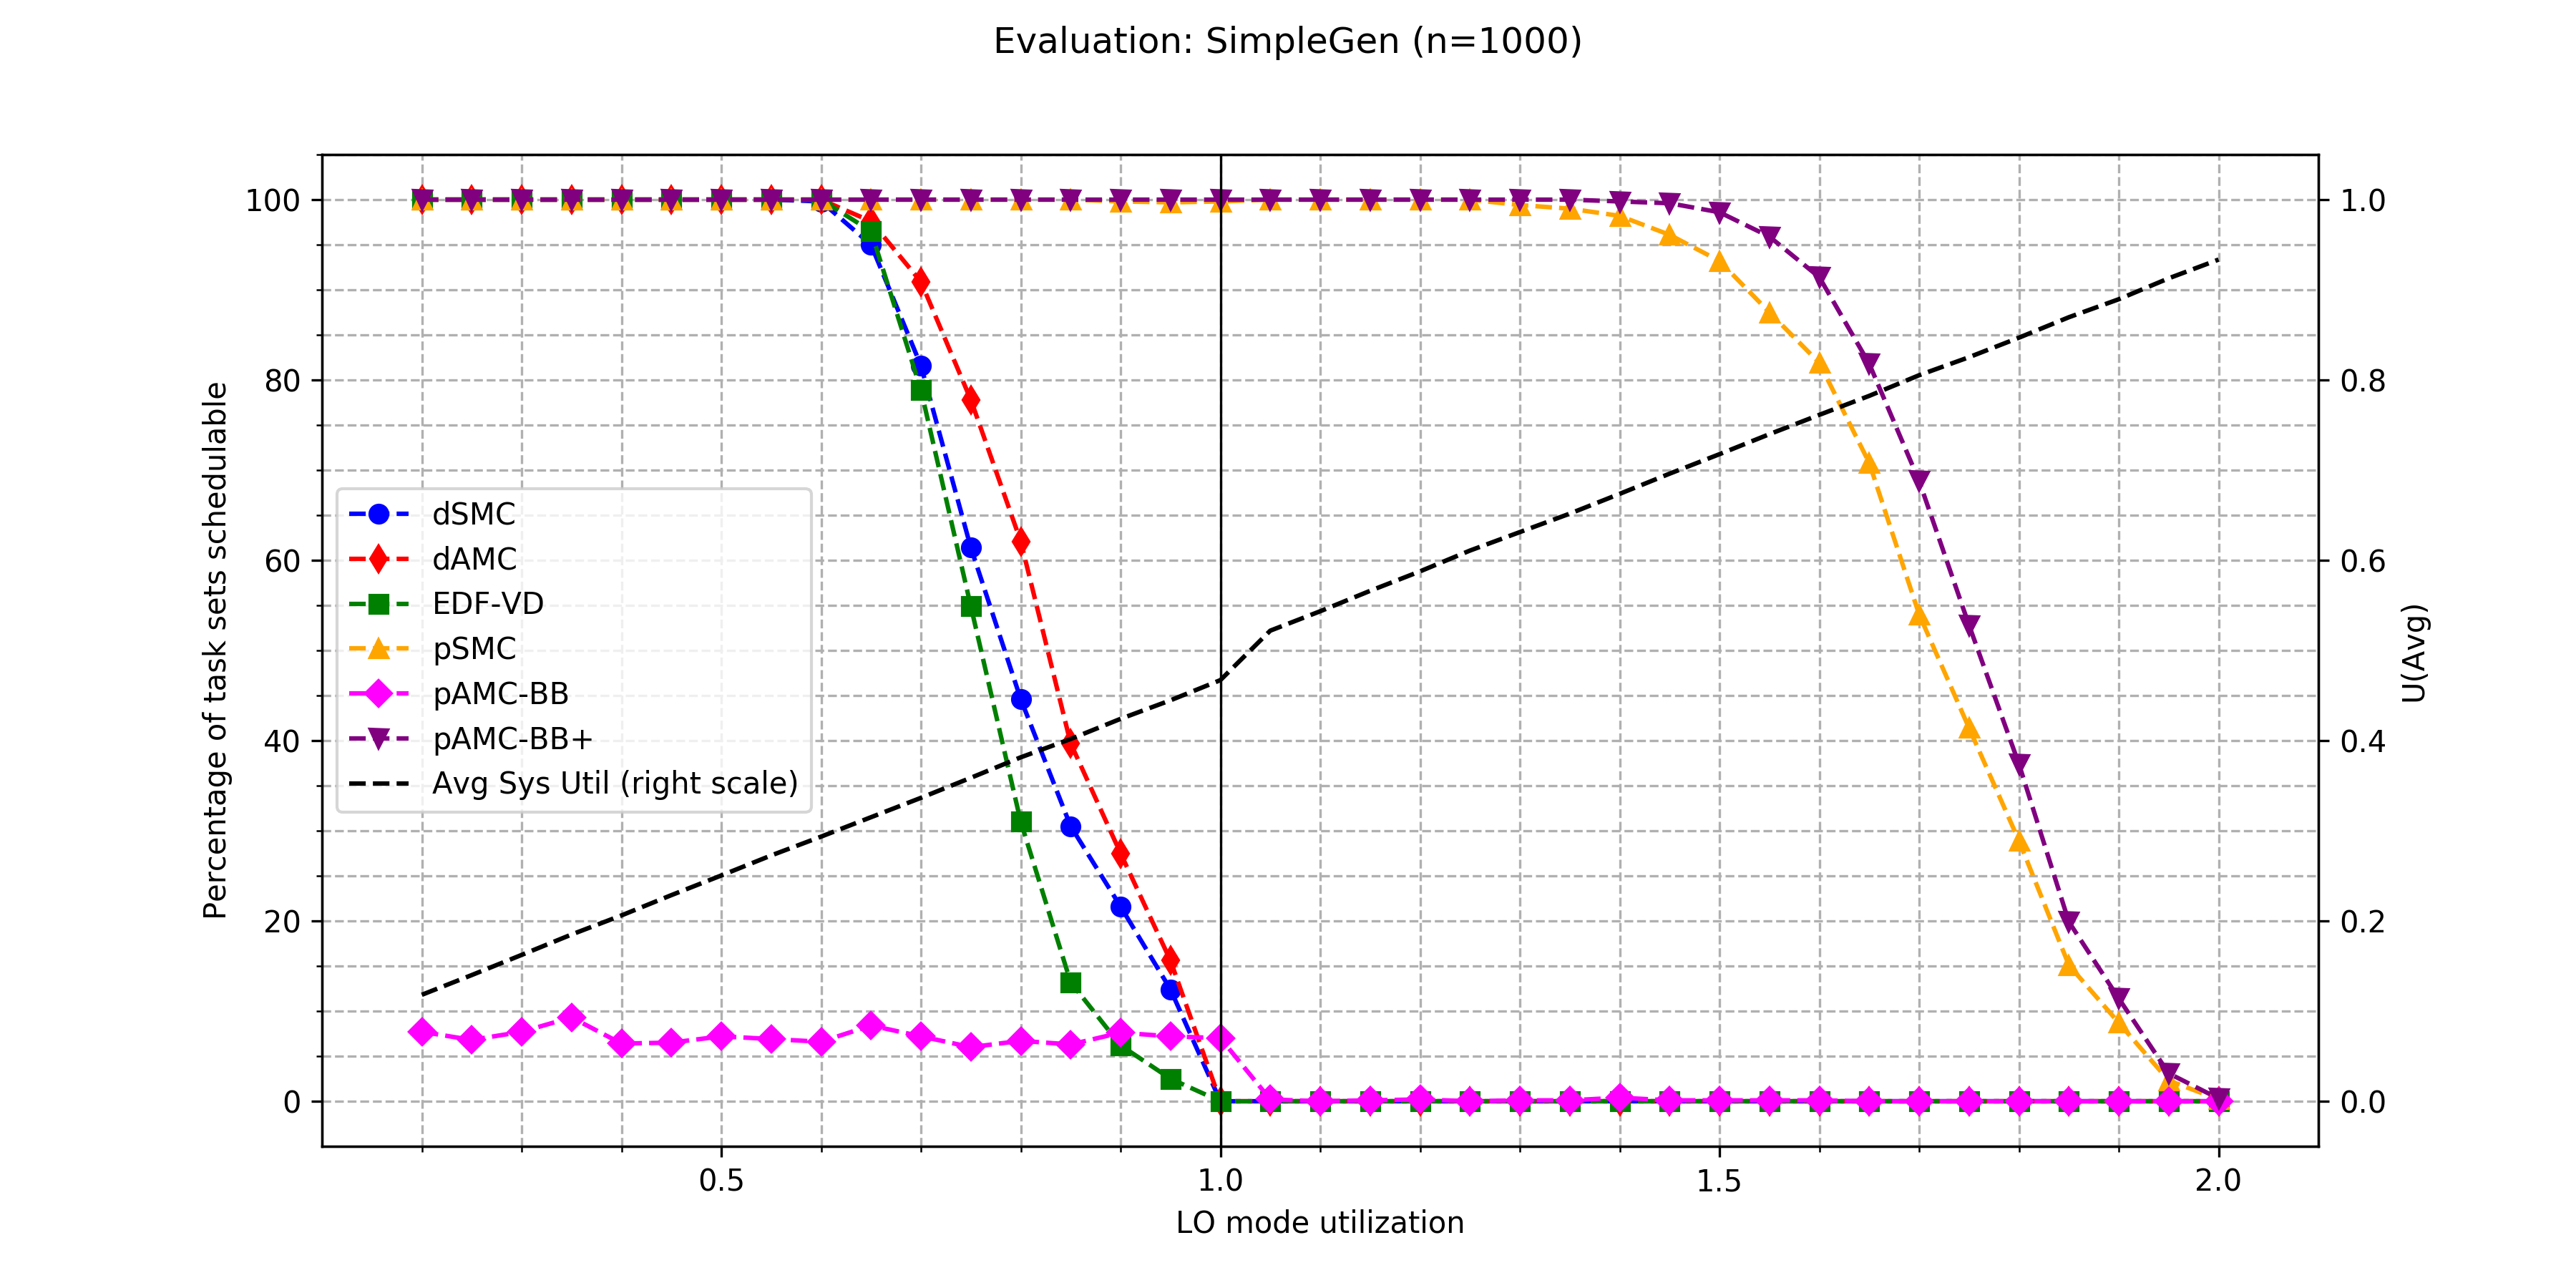
\includegraphics[width=1.3\textwidth]{figures/schedulability_rates_simplegen.png}}
        \caption{}\label{subfig:eval-schemes-simplegen}
    \end{subfigure}
    \newline
    \newline
    \newline
    \begin{subfigure}[c]{\textwidth}
        \makebox[\textwidth][c]{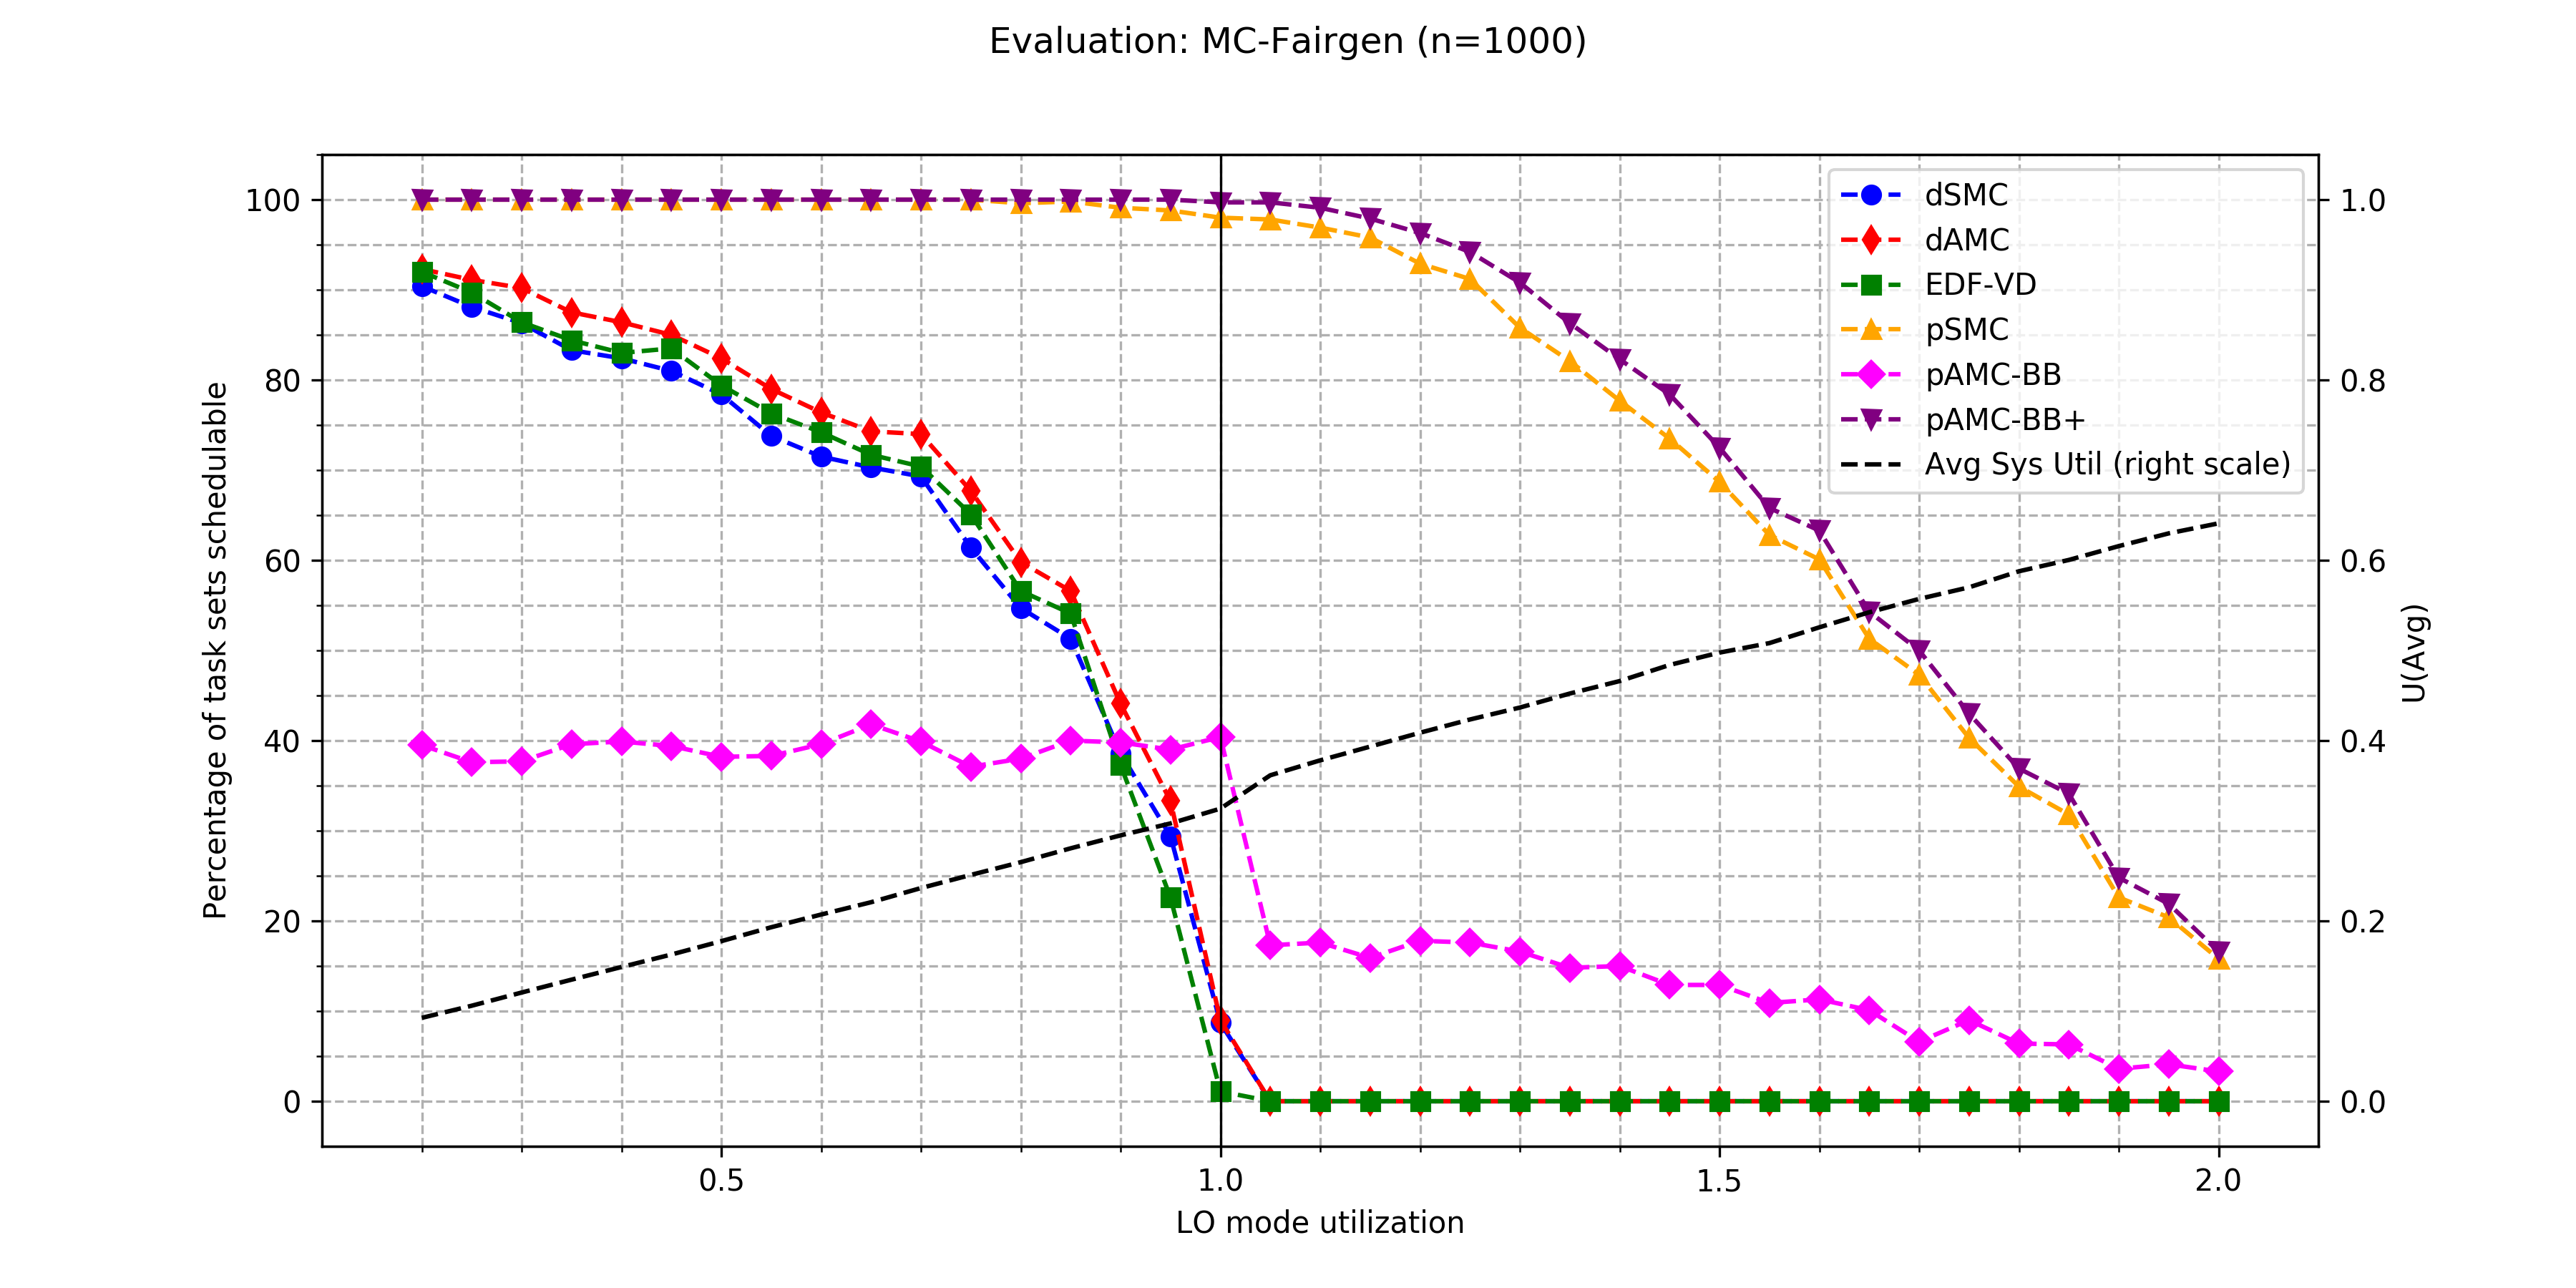
\includegraphics[width=1.3\textwidth]{figures/schedulability_rates_fairgen.png}}
        \caption{}\label{subfig:eval-schemes-fairgen}
    \end{subfigure}
    \caption{}\label{fig:eval-schemes}
\end{figure}



\newpage
\subsection{Monte Carlo Test Schemes}
We also can compare the Monte-Carlo-based schemes to their theoretical counterparts. \Cref{fig:eval-monte-carlo} displays the resulting rates. Again, the same 1000 task sets from \cref{subfig:eval-schemes-fairgen} were tested for each data point. As described in  \cref{subsec:monte-carlo-schemes}, lower DMP thresholds have to be applied for comparable results; they were chosen at $10^{-3}$ and $10^{-4}$ for LO- and HI-critical tasks, respectively. Both Monte-Carlo methods simulated 10'000 hyperperiods for every task set. Duration of the black box state was again assumed to be one hyperperiod.

Both Monte-Carlo schemes matched the results of their counterpart fairly closely. However, their computation is far more expensive (\cref{sec:performance}), thus they serve more as proof of concept.
\begin{figure}[ht]
    \makebox[\textwidth][c]{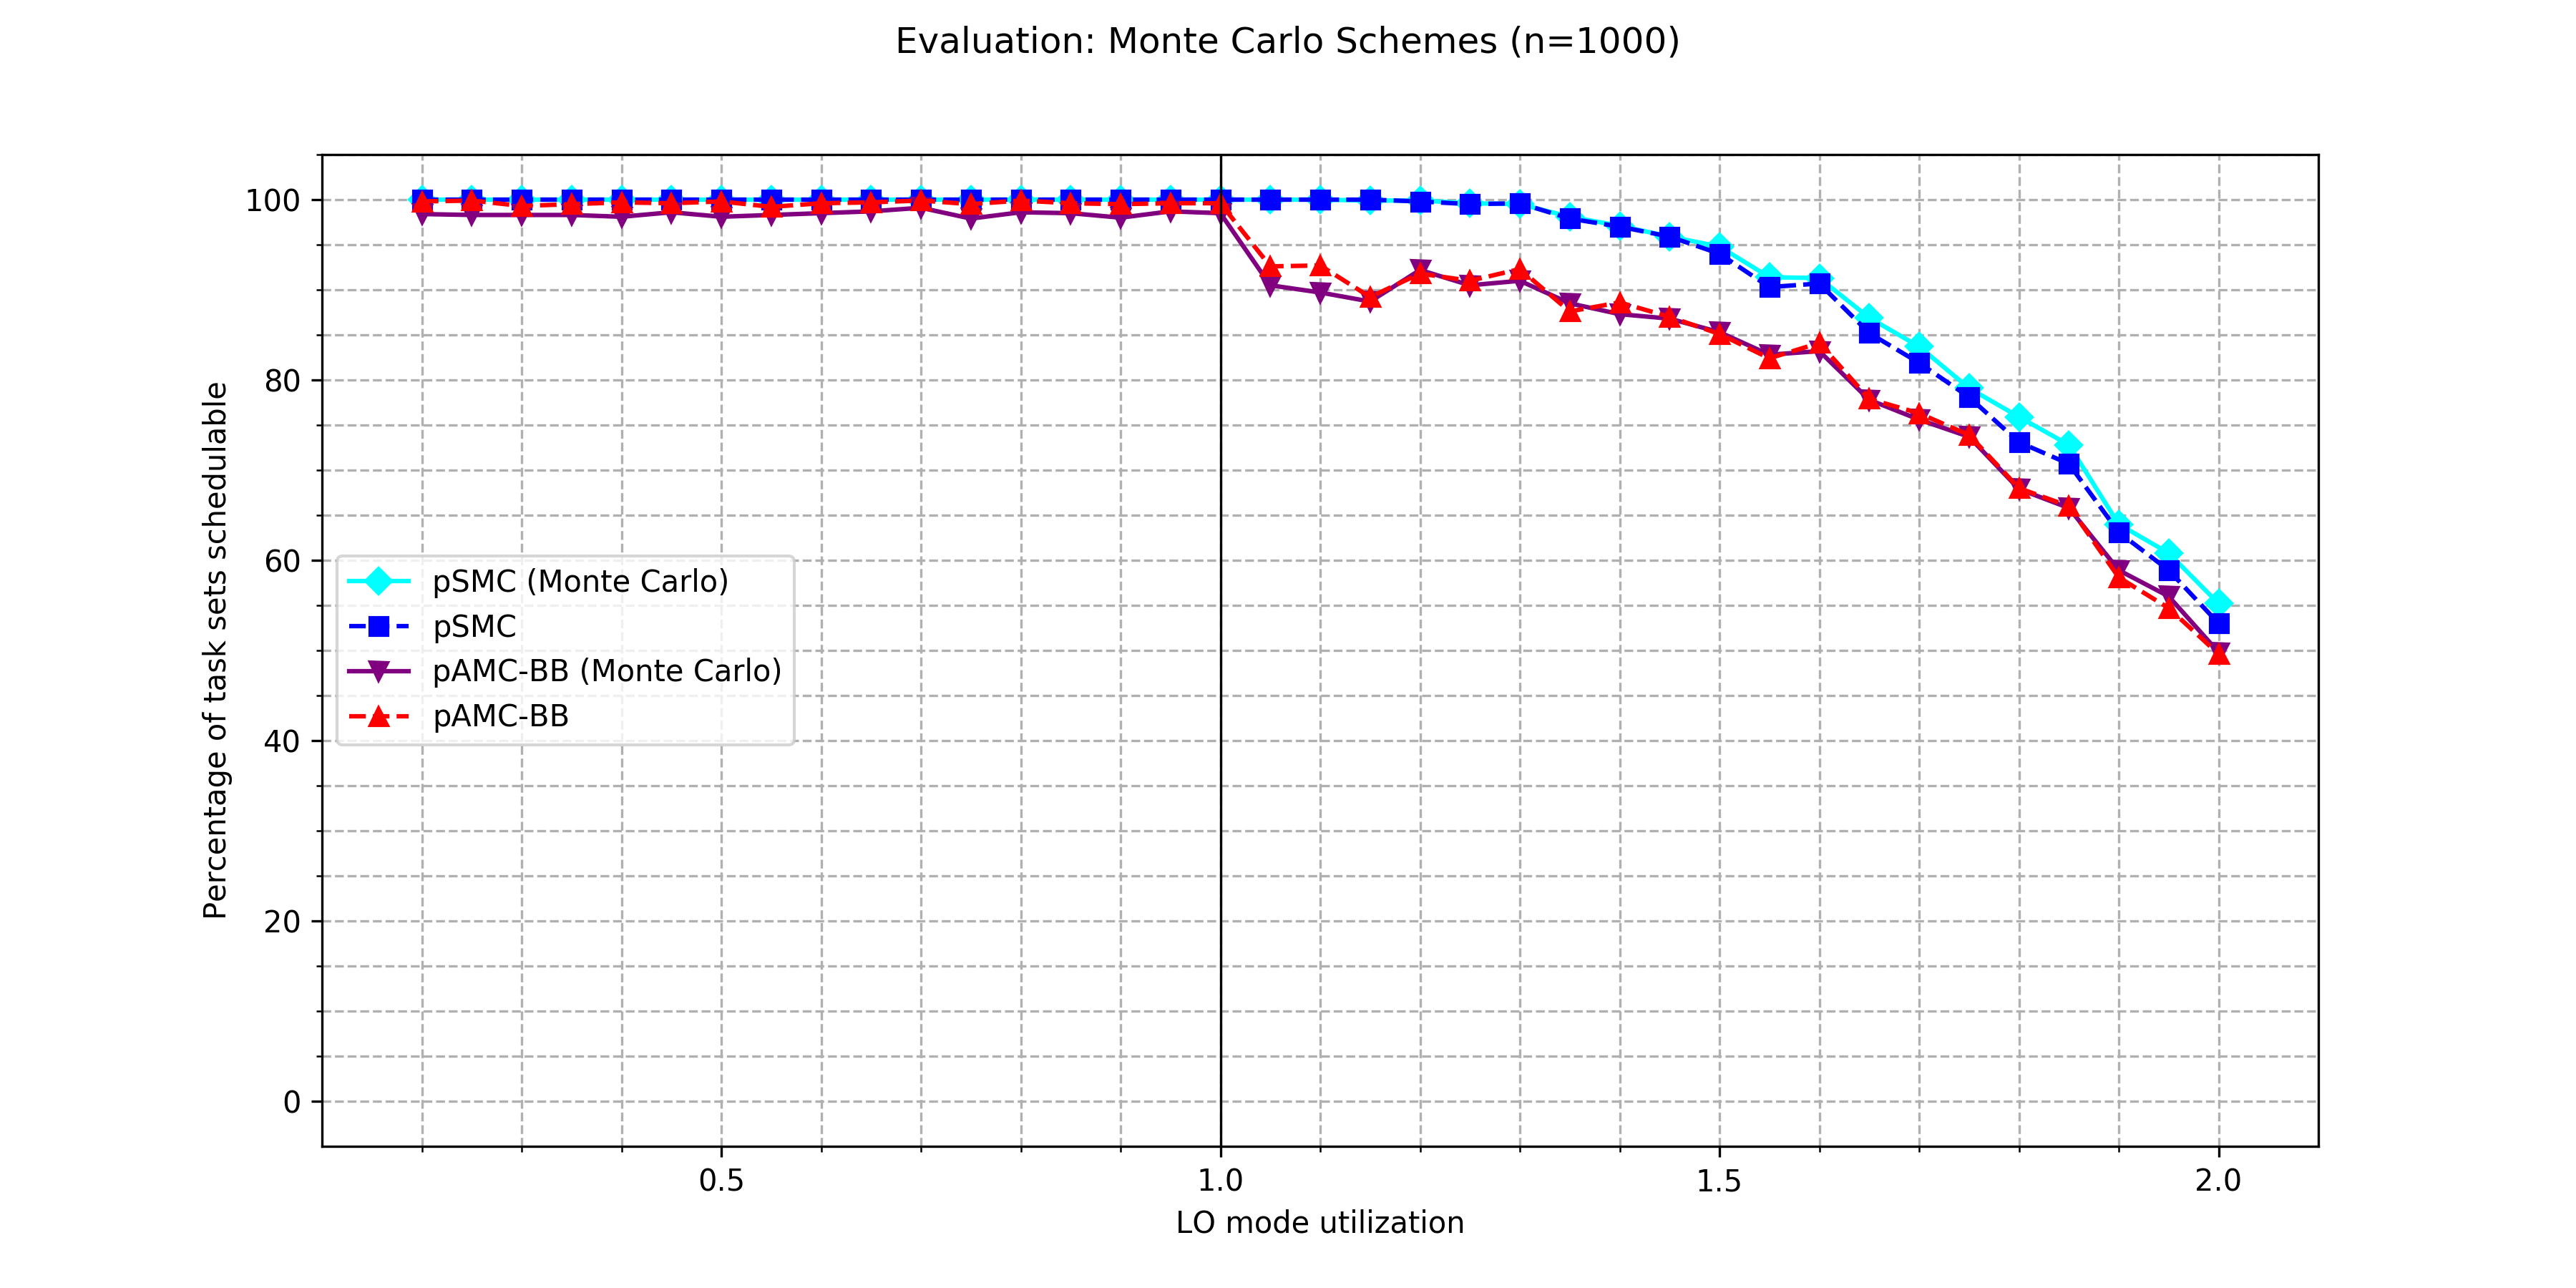
\includegraphics[width=1.3\textwidth]{figures/schedulability_rates_monte_carlo.png}}
    \caption{}\label{fig:eval-monte-carlo}
\end{figure}


\newpage
\section{Performance}
\label{sec:performance}

\subsection{Computation Times}
\Cref{tbl:computation-times} shows time measurements for computations performed in \cref{sec:eval-schemes}. These measurements were taken on an Intel i5-7600K, 4 cores @ 3.80 GHz, with 16 GB of RAM.
\begin{table}[ht]
    \centering
    \caption{Computation times, number of tasks = 1000}
    \label{tbl:computation-times}
    \begin{tabular}{@{}lll@{}}
        \toprule
        Plot & Method & Average time measured [s] \\ \midrule
        \cref{subfig:eval-schemes-simplegen} & Task Set Synthesis & 35.765 \\
        & dSMC & 18.066 \\
        & dAMC & 18.117 \\
        & EDF-VD & 17.957 \\
        & pSMC & 2354.446 (39min 14s) \\
        & pAMC-BB & 2012.072 (33min 32s) \\
        & pAMC-BB+ & 2098.982 (34min 59s) \\
        \midrule
        \cref{subfig:eval-schemes-fairgen} & Task Set Synthesis & 41.546 \\
        & dSMC & 10.994 \\
        & dAMC & 11.038 \\
        & EDF-VD & 10.922 \\
        & pSMC & 1884.353 (31min 24s) \\
        & pAMC-BB & 1477.216 (24min 37s) \\
        & pAMC-BB+ & 1494.017 (24min 54s) \\
        \midrule
        \cref{fig:eval-monte-carlo} & pSMC & 1623.465 (27min 3s) \\
        & pSMC (Monte Carlo) & 37305.045 (10h 21min 45s) \\
        & pAMC-BB & 1482.949 (24min 43s) \\
        & pAMC-BB (Monte Carlo) & 43601.306 (12h 6min 41s) \\
    \end{tabular}
\end{table}

\subsection{Multiprocessing}
As described in \cref{sec:eval-mod}, all schedulability test scripts make use of Python's \texttt{multiprocessing} library. See \cref{tbl:speedup} for the speedups gained using multiple processes. Note that parallelization actually has a negative impact for the lighter-weight deterministic tests. For the other, more complex tests, however, speedup scales quite well with the number of cores. Since the problem set can be split up in fairly fine-grained parts (up to a single task set being tested), this should also scale well with larger architectures.

\begin{table}[ht]
    \centering
    \caption{Speedups achieved with multiprocessing (4 cores)}
    \label{tbl:speedup}
    \begin{tabular}{@{}llll@{}}
        \toprule
        Method & Sequential time $t_1$ & Parallel time $t_4$ & Speedup $\frac{t_1}{t_4}$ \\ \midrule
        dSMC & 1.590s & 30.900s & 0.051 \\
        dAMC & 1.971s & 25.169s & 0.078 \\
        EDF-VD & 0.318s & 25.909s & 0.012 \\
        pSMC & 5903.575s & 1646.722s & 3.585 \\
        pAMC-BB & 5370.185s & 1503.402s & 3.572 \\
        pAMC-BB+ & 5376.428s & 1515.235s & 3.548 \\
        Total & 16654.066s & 4747.436s & 3.508 \\
    \end{tabular}
\end{table}


%%%%%%%%%%%%%%%%%%%%%%%%%%%%%%%%%%%%%%%%%%%%%%%%%%%%%%%%%%%%%%%%%%
\chapter{Conclusion}
\label{cha:conclusion}
In this chapter, I revisit the framework's main attributes to conclude on this thesis, and outline some possibilities for its future.

\section{Summary}
The main goal of this thesis was more about reviewing and compiling existing work and then integrating it into a common platform, and less about assessing and comparing different synthesis methods or schedulability tests in detail. The resulting framework's objects, scripts, and functions provide a skeleton, with which new ideas can quickly be implemented and evaluated. My focus was to write code that is \textbf{a)} well documented, so other people can understand and use it quickly, \textbf{b)} extensible, so future work can be integrated without having to overhaul a majority of the existing code base, and \textbf{c)} fast, producing meaningful results in little time by fully utilizing all available CPU cores.

\section{Future Work}
Although I have tried to implement a wide spectrum of different test schemes and even explored possibilities beyond mixed-criticality scheduling, this framework is still only at its very beginning. What follows are some ideas for future expansions.
\begin{itemize}
    \item \textbf{Fair stochastic task sets:} Our method of combining deterministic mixed-criticality task sets and random probability distributions may be too simple. The fairness properties presented in \cite{ramanathan2016evaluation} may also have to cover task execution time distributions to be applicable in stochastic analysis.
    \item \textbf{Real task sets:} Task sets from the "real world" could be investigated further, either directly parsing them for schedulability testing (building a task set "library"), or also creating a new synthesis heuristic based on their features.
    \item \textbf{Response time analysis for dynamic-priority systems:} Similar to my response time analysis implementation (\cref{subsec:backlog-comp}) for fixed-priority scheduling, there exists a variation designed for dynamic priorities as well, described in \cite{diaz2002probabilistic}. 
    \item \textbf{Probabilistic HI-mode analysis:} In the probabilistic schemes presented here, HI-mode has been replaced by a black box or not considered at all. More sophisticated schedulability schemes that also analyze HI-mode need to be developed and possibly implemented here.
    \item \textbf{Arbitrary criticality levels:} The framework and all synthesis and analysis schemes could be enhanced to support $n$ different criticality levels as opposed to only $LO$ and $HI$.
    \item \textbf{Related topics:} \Cref{cha:energy} provides an entry point to a related topic just as diverse as mixed-criticality. The \texttt{energy} module is only thought as a teaser and would probably be worth an entire thesis in itself, when expanded. Besides that, applications in other topics for parts of the framework such as convolution and shrinking could be explored.
\end{itemize}

\bibliographystyle{abbrv}
\bibliography{references} 

\begin{appendices}
\chapter{Final Presentation}
\chapter{Certificate of Originality}
\chapter{Codebase}
All source code files as well as other documents and data involved in this thesis are available online under \url{https://github.com/luca-stalder/bsc-thesis}. See the read-me file contained there for further details.
\end{appendices}

\end{document}